\chapter{Algorytm diagnozowania skoliozy}
\label{chap:skolioza}

\section{Kliniczna charakterystyka skoliozy}
Skolioza opisywana jest w literaturze medycznej jako jedno lub więcej nieprawidłowych bocznych skrzywień kręgosłupa z rotacją kręgów lub bez.
Według Scoliosis Research Society skoliozę określa się jako skrzywienie kręgosłupa o kąt Cobba większy niż 10\degree{}.
Na zdjęciu rentgenowskim kręgosłup osoby cierpiącej na skoliozę wygląda bardziej jak litera ``S'' lub ``C'' niż prosta linia\cite{srs}.
Termin ``skolioza'' ma swoje korzenie w starożytnym słowie ``skolios'' (wygięty, skrzywiony) i został po raz pierwszy użyty przez Galena (130-201 rok naszej ery)\cite{koniecznymr}.

Skoliozę można podzielić na typy: idiopatyczną, wrodzoną i nerwowo-mięśniową.
Najczęstsza postać skoliozy czyli idiopatyczna skolioza młodzieńcza (AIS), ma nieznaną przyczynę co odzwierciedla termin ``idiopatyczna''.
AIS jest zazwyczaj wykrywane w okresie dzieciństwa i dorastania, zwłaszcza w okresach szybkiego wzrostu.
Skolioza wrodzona jest spowodowana nieprawidłowym rozwojem kręgosłupa w stadium embrionalnym, co może obejmować brak segmentacji kręgów, nieprawidłowy kształt lub nieprawidłową liczbę kręgów.
Ten rodzaj skoliozy jest często związany z czynnikami genetycznymi i może współistnieć z innymi wadami wrodzonymi, dlatego zazwyczaj rozpoznaje się go po urodzeniu lub we wczesnym okresie niemowlęcym\cite{lim}.
Skolioza nerwowo-mięśniowa jest wynikiem zaburzeń nerwowo-mięśniowych, które wpływają na mięśnie i nerwy odpowiedzialne za utrzymanie prawidłowego ułożenia kręgosłupa.
Do najczęstszych przyczyn należą: porażenia mózgowe, dystrofia mięśniowa i urazy rdzenia kręgowego\cite{yale}.

Skolioza jest najczęstszym schorzeniem kręgosłupa wśród dzieci i młodzieży.
Według różnych badań częstość występowania skoliozy idiopatycznej młodzieńczej w tym wieku wynosi od 0,47\% do 5,2\%..
Stosunek liczby dziewcząt do chłopców waha się od 1,5:1 do 3:1 i znacznie wzrasta wraz z wiekiem\cite{koniecznymr}.

Diagnoza skoliozy wymaga wieloetapowego podejścia łączącego badanie kliniczne z diagnostyką obrazową.
Istotne jest wczesne wykrycie i ocena stopnia zaawansowania choroby, szczególnie w przypadku AIS.
Proces diagnostyczny rozpoczyna się od zebrania dokładnej historii pacjenta obejmującej:
\begin{itemize}
    \item dynamikę wzrostu dziecka w ostatnim czasie,
    \item ból pleców,
    \item rodzinną historia skoliozy.
\end{itemize}

Test zgięcia Adama służy do wykrywania strukturalnych deformacji kręgosłupa, w szczególności rotacji kręgów i wynikającego z tego garbu żebrowego lub wypukłości lędźwiowej.
Jest podstawową metodą przesiewową stosowaną zarówno przez lekarzy ortopedów, jak i fizjoterapeutów oraz w badaniach populacyjnych u dzieci i młodzieży.
Test zgięcia jest bardzo czuły na deformacje rotacyjne, ale nie pozwala na ustalenie wartości kąta skrzywienia.
Dlatego stanowi wstęp zarówno do oceny klinicznej skoliometrem, jak i do ewentualnej diagnostyki obrazowej.

Pomiar skoliozy skoliometrem stanowi uzupełnienie testu zgięcia Adama i pozwala na półilościową ocenę wielkości rotacji tułowia (Angle of Trunk Rotation – ATR).
Badanie wykonuje się w pozycji pochylenia do przodu, przykładając skoliometr w linii wyrostków kolczystych na poziomie największej deformacji.
Urządzenie rejestruje różnicę wysokości obu stron tułowia, co odzwierciedla stopień rotacji kręgów.
Wartości ATR powyżej 5–7 stopni są sygnałem do pogłębionej diagnostyki, a powyżej 10 stopni zazwyczaj wymagają wykonania badania obrazowego, najczęściej RTG, wraz z oceną kąta Cobba.
Pomiar skoliometrem jest szybki, nieinwazyjny i szeroko stosowany zarówno w badaniach przesiewowych, jak i w monitorowaniu progresji skrzywienia.\cite{czaprow}

Radiogram kręgosłupa stanowi podstawowe narzędzie obrazowe wykorzystywane w ocenie skoliozy, a szczególnie w ilościowej analizie deformacji czołowej metodą Cobba.
Standardem jest wykonanie projekcji PA (tylno-przedniej) całego kręgosłupa w pozycji stojącej, co umożliwia uwzględnienie obciążenia grawitacyjnego i realistyczną ocenę stopnia skrzywienia.
Istotne jest zachowanie odpowiednich parametrów ekspozycji oraz minimalizacja artefaktów wynikających z rotacji ciała lub niewłaściwego ustawienia pacjenta.
Mimo że badanie RTG jest dwuwymiarowe i niesie ograniczenia w ocenie rotacji osiowej, pozostaje metodą referencyjną w diagnostyce skoliozy ze względu na wysoką dostępność, powtarzalność oraz możliwość precyzyjnego wyznaczenia kąta skrzywienia.

Przed przystąpieniem do pomiaru kąta Cobba konieczna jest dokładna analiza obrazu RTG w celu wyznaczenia kręgów zaangażowanych w deformację.
Najpierw identyfikuje się kręg szczytowy, czyli kręg o największym odchyleniu bocznym od osi pionowej.
Następnie wyznacza się kręgi krańcowe górny i dolny - charakteryzujące się największym nachyleniem płytek granicznych względem poziomu.
Wybór tych struktur jest kluczowy, ponieważ stanowi punkt wyjścia dla dalszych konstrukcji geometrycznych pomiaru.

Pomiar kąta Cobba polega na konstrukcji prostych geometrycznych prowadzonych względem płytek granicznych kręgów krańcowych.
Najpierw rysuje się linię styczną do górnej powierzchni kręgu krańcowego górnego oraz linię styczną do dolnej powierzchni kręgu krańcowego dolnego.
Następnie prowadzi się prostopadłe do tych linii, które po przedłużeniu przecinają się, tworząc charakterystyczny kąt odpowiadający wielkości skrzywienia.
W przypadku gdy linie płytkowe przecinają się w obrębie pola obrazu, dopuszczalne jest bezpośrednie mierzenie kąta między nimi.
Pomiar powinien być wykonywany z zachowaniem jednolitej techniki, ponieważ metoda Cobba wykazuje pewien poziom zmienności obserwatora\cite{gstoettner}.
Dla celów monitorowania progresji skoliozy kluczowe jest zatem stosowanie tej samej procedury pomiarowej, najlepiej przez tego samego obserwatora, oraz opieranie się na badaniach wykonanych w analogicznych warunkach ekspozycji i pozycjonowania.

Wartość kąta Cobba stanowi podstawowy parametr ilościowy determinujący rozpoznanie skoliozy, ocenę jej nasilenia oraz dobór strategii terapeutycznej.
Kąt poniżej 10\degree{} traktuje się jako asymetrię tułowia, natomiast wartości równe lub przekraczające 10\degree{} stanowią kryterium rozpoznania skoliozy.
Zakres 10--25\degree{} zwykle kwalifikuje pacjenta do obserwacji i leczenia zachowawczego, natomiast skrzywienie 25--45\degree{} u pacjentów rosnących stanowi wskazanie do leczenia gorsetowego.
Deformacje przekraczające 45--50\degree{} rozważa się w kontekście leczenia operacyjnego, zwłaszcza w przypadku progresji\cite{negrini_sosort, kuznia}.
Metoda Cobba odgrywa również istotną rolę w ocenie dynamiki skrzywienia -- progresja o więcej niż 5\degree{} pomiędzy kolejnymi badaniami RTG uznawana jest za klinicznie istotną\cite{kuznia}.
Dzięki swojej prostocie i wysokiej reprodukowalności parametr ten pozostaje podstawą planowania i monitorowania leczenia skoliozy we wszystkich postaciach.

Kliniczny standard pomiaru kąta Cobba opiera się na zdjęciu RTG wykonanym w pozycji stojącej.
Niniejsza praca proponuje automatyzację analogicznego pomiaru na podstawie trójwymiarowej segmentacji badania MRI.
Podejście to zachowuje matematyczną definicję metody Cobba, eliminując jednocześnie konieczność ręcznego wskazywania kręgów krańcowych przez radiologa.

Należy jednak podkreślić istotną różnicę metodologiczną między klinicznym standardem a podejściem zaproponowanym w niniejszej pracy.
Radiogram wykonywany jest w pozycji stojącej, podczas gdy badanie MRI, stanowiące źródło analizowanych segmentacji, przeprowadza się zazwyczaj w pozycji leżącej.
Brak obciążenia osiowego w pozycji leżącej sprawia, że skrzywienie bywa mniej nasilone niż w staniu, co może prowadzić do systematycznego zaniżenia mierzonej wartości kąta względem standardu radiologicznego.
Z tego powodu wynik uzyskany proponowaną metodą należy traktować jako miarę spójną wewnętrznie, użyteczną w szczególności do oceny przesiewowej i porównań, a nie jako wartość bezpośrednio równoważną pomiarowi z radiogramu stojącego.
Jednocześnie analiza oparta na trójwymiarowej segmentacji eliminuje błąd rzutowania właściwy dwuwymiarowemu radiogramowi, co stanowi potencjalną przewagę nad klasycznym pomiarem.

\section{Założenia funkcjonalne i niefunkcjonalne}
W celu zrealizowania postawionego celu pracy zdefiniowano szereg wymagań funkcjonalnych oraz niefunkcjonalnych.

Wymagania funkcjonalne:

\begin{itemize}
    \item \textbf{Obsługa wejściowych danych wolumetrycznych} -- system musi umożliwiać wczytanie trójwymiarowych obrazów medycznych (mapy segmentacji) w standardzie NIfTI\cite{nifti} (.nii.gz), reprezentujące odcinek lędźwiowy kręgosłupa wraz z kanałem kręgowym.
    \item \textbf{Wyznaczenie linii środkowej kanału kręgowego} -- algorytm musi wygenerować gładką krzywą reprezentującą przebieg kanału kręgowego w przestrzeni 3D.
    \item \textbf{Lokalna analiza geometrii kręgu} -- dla każdego kręgu system wyznacza lokalny układ współrzędnych.
    \item \textbf{Ekstrakcja przekrojów 2D} -- algorytm dokonuje próbkowania (resampling) wolumenu do płaszczyzny strzałkowej każdego kręgu.
    \item \textbf{Wyznaczenie punktów charakterystycznych} -- algorytm określa cztery narożne punkty trzonów kręgów
    \item \textbf{Automatyczny pomiar kąta Cobba} -- system oblicza kąt Cobba pomiędzy dowolnymi parami kręgów oraz identyfikuje parę kręgów o największej deformacji.
    \item \textbf{Określenie strony skrzywienia} -- system klasyfikuje skrzywienie jako prawo- lub lewostronne.
    \item \textbf{Wizualizacja i eksport wyników} -- system musi generować dane wynikowe i pośrednie w formacie umożliwiającym ich wizualną weryfikację przez lekarza (np. pliki znaczników JSON kompatybilne z oprogramowanie 3D Slicer), zawierające punkty, linie pomiarowe oraz wektory.
\end{itemize}

Wymagania niefunkcjonalne:
\begin{itemize}
    \item \textbf{Odporność na nieciągłość danych} -- algorytm powinien radzić sobie z przerwami w segmentacji kanału kręgowego.
    \item \textbf{Powtarzalność wyników} -- dla tych samych danych wejściowych algorytm musi zwracać zawsze ten sam wynik pomiarowy.
    \item \textbf{Pełna automatyzacja} -- proces pomiaru musi przebiegać bez interakcji manualnej, w szczególności bez ręcznego wskazywania kręgów krańcowych przez użytkownika.
    \item \textbf{Efektywność czasowa przetwarzania} -- algorytm musi charakteryzować się niską złożonością obliczeniową, umożliwiając przetworzenie pojedynczego badania w czasie akceptowalnym klinicznie.
    \item \textbf{Interoperacyjność} -- rozwiązanie powinno wykorzystywać otwarte standardy wymiany danych medycznych, co pozwala na łatwą integrację z istniejącymi narzędziami badawczymi oraz narzędziami do wizualizacji i analizy obrazów medycznych (np. 3D Slicer).
\end{itemize}
Zdefiniowane powyżej wymagania stanowią podstawę do opracowania metodyki oraz implementacji algorytmu, które zostaną przedstawione w kolejnych rozdziałach pracy.


\section{Metodyka i opis algorytmu}
W niniejszym rozdziale przedstawiono opis zaprojektowanego algorytmu. Proces przetwarzania danych podzielono na etapy: od wstępnego przetwarzania obrazu (preprocessing), poprzez ekstrakcję cech geometrycznych, aż po finalne obliczenia pomiarów wynikowych.

\begin{figure}[H]
    \centering
    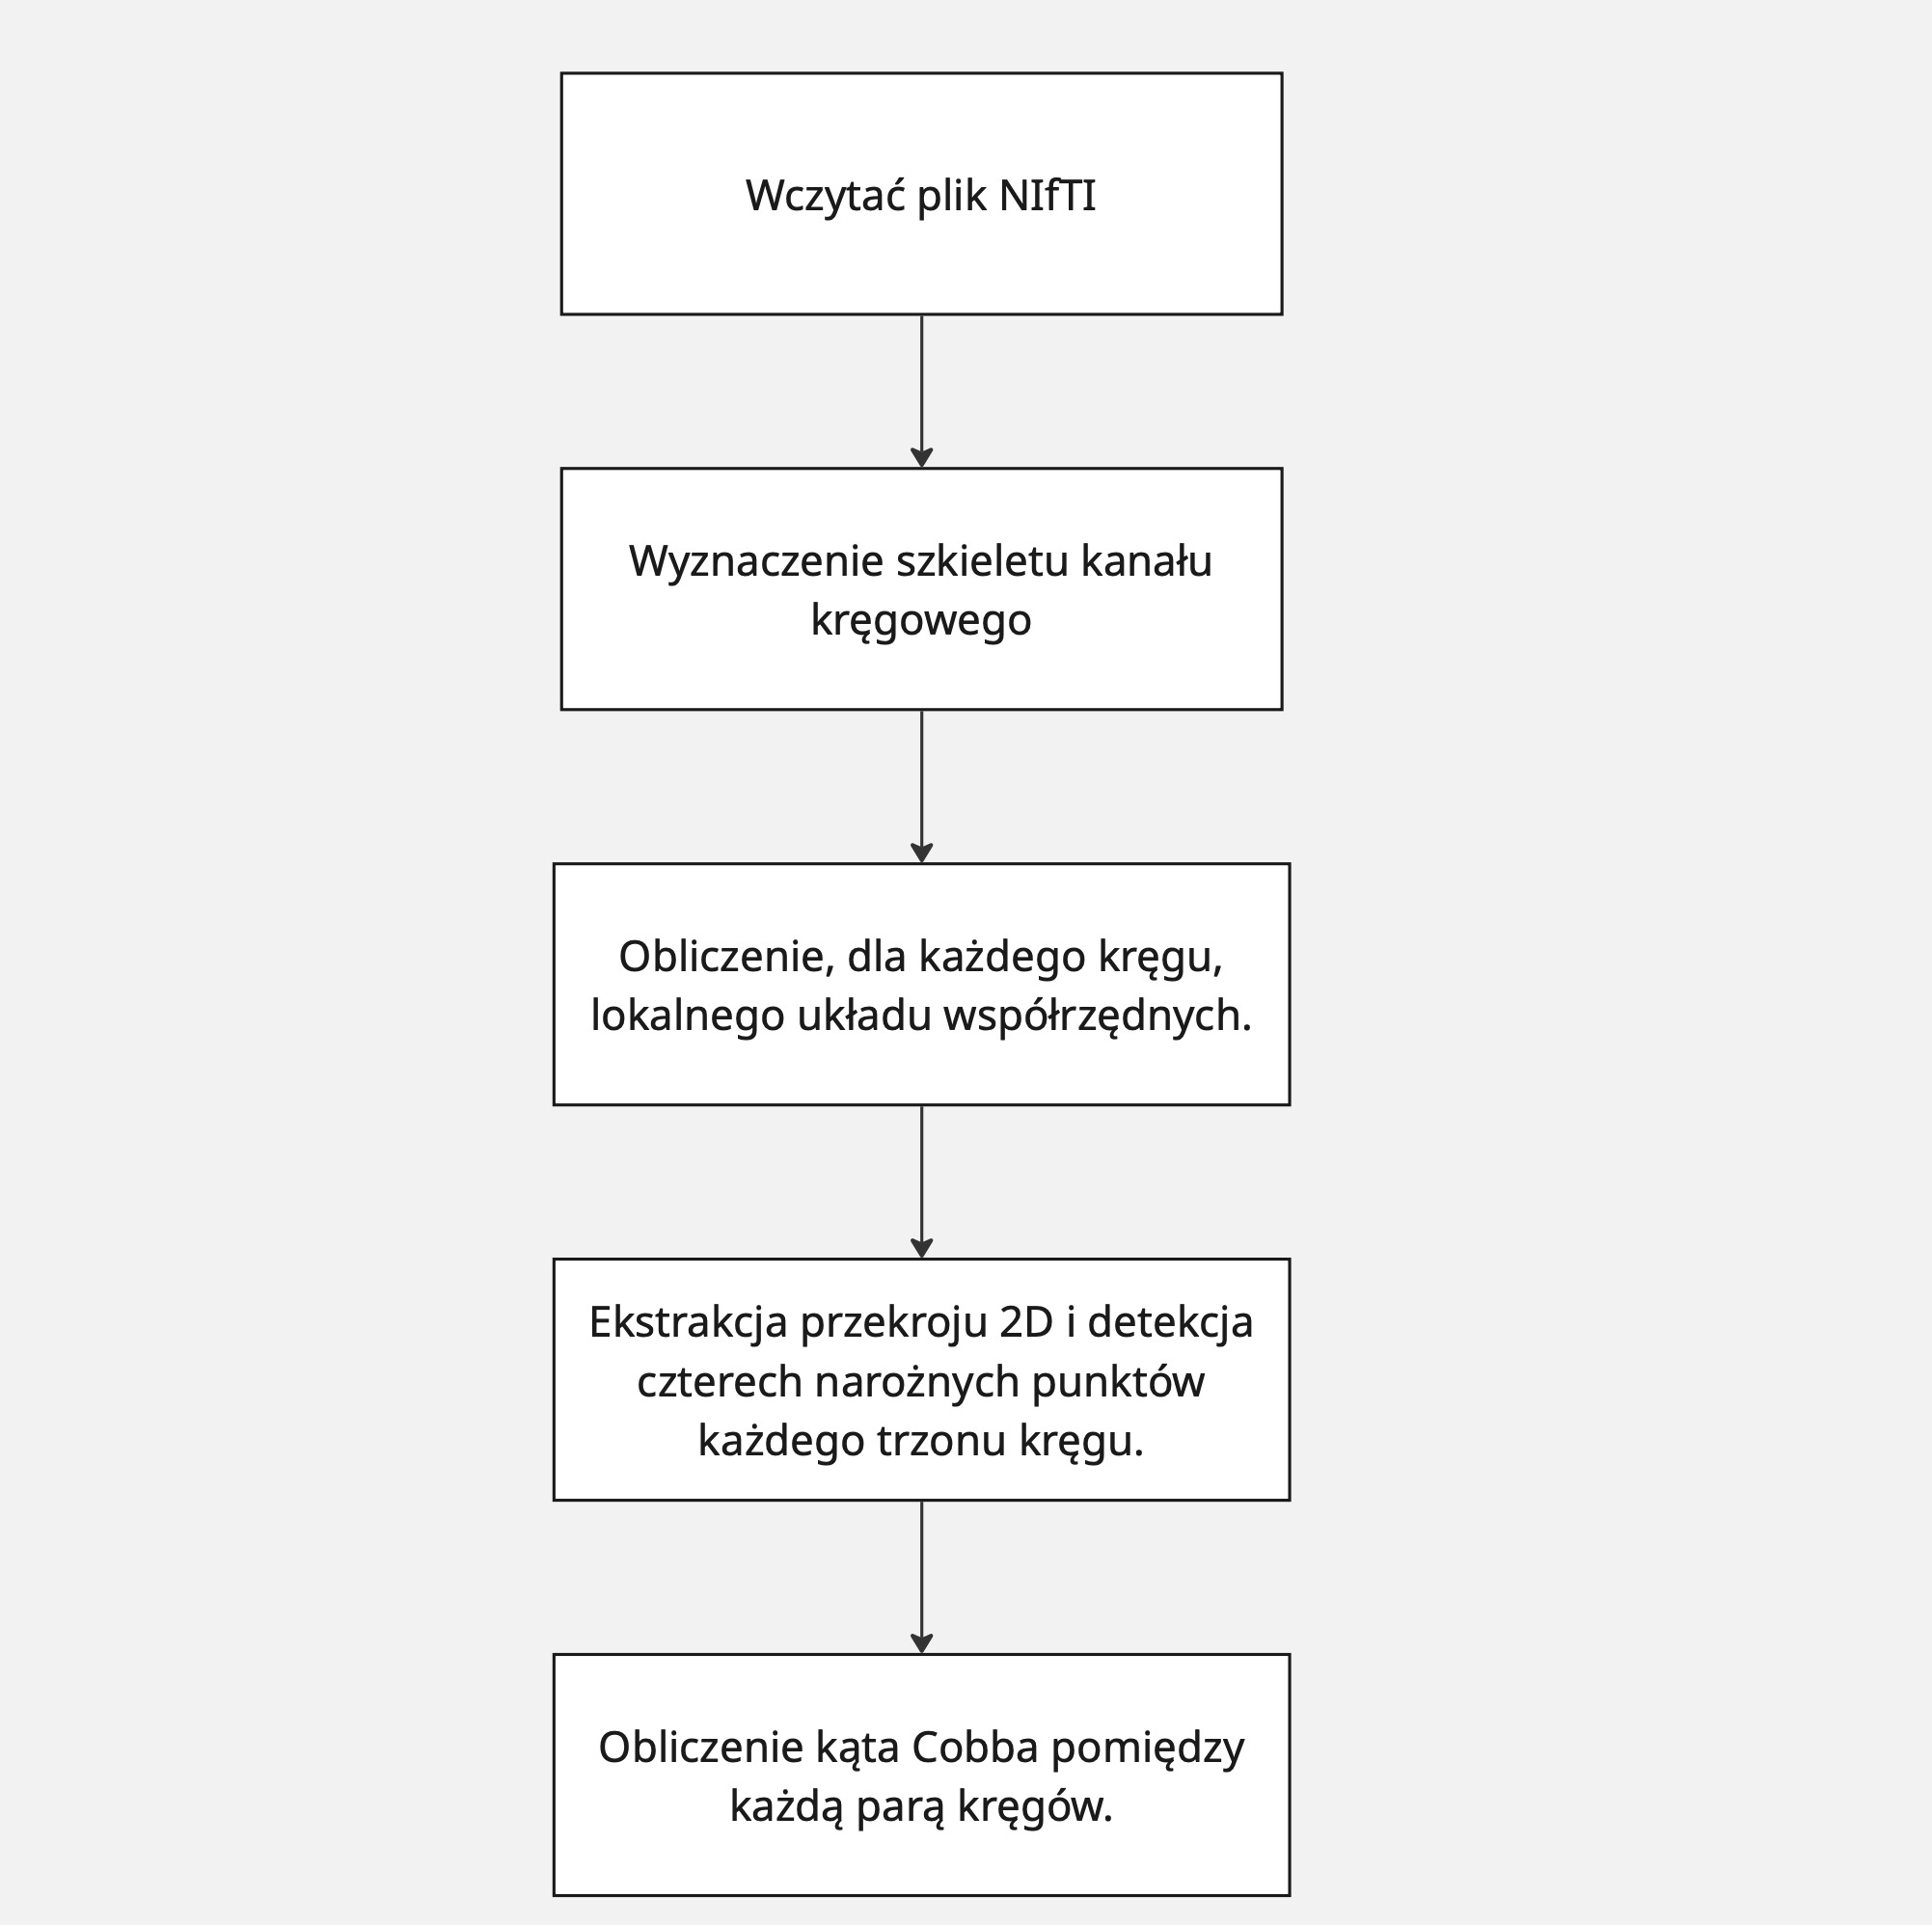
\includegraphics[width=1\textwidth]{obrazy/scoliosis_pipeline.jpg}
    \captionsetup{justification=centering, font=small}
    \caption{Ogólny potok przetwarzania danych dla algorytmu detekcji skoliozy}
    \label{fig:scoliosis-pipeline}
\end{figure}

\subsection{Wyznaczenie i rekonstrukcja linii środkowej kanału kręgowego}
\label{subsec:centerline}
Pierwszym krokiem algorytmu jest wyznaczenie szkieletu kanału kręgowego.
Metoda zaczyna się od połączenia w jedną całość trzech etykiet segmentacji składających się na kanał kręgowy: właściwego kanału kręgowego, ogona końskiego oraz worka oponowego.
W ten sposób obszar kanału kręgowego staje się bardziej odporny na „przerwy" w segmentacji, co zwiększa obszar dostępny do dalszego przetwarzania.

Następnym krokiem jest przekazanie złączonych etykiet do funkcji \texttt{skeletonize} z argumentem \texttt{method='lee'} z pakietu \texttt{scikit-image} w celu wyznaczenia szkieletu kanału kręgowego\cite{scikit-skeletonize}.
Następnie na zwróconym zbiorze pikseli (szkielecie) dokonano przepróbkowania (resamplingu) do przestrzeni wejściowego kanału kręgowego.
Kolejnym krokiem jest przeiterowanie się przez całą długość wektora Z (wysokość) przepróbkowanego szkieletu kanału kręgowego z krokiem równym grubości warstwy przestrzeni i wyznaczenie punktów kanału kręgowego.
Niekiedy segmentacja kanału kręgowego mimo połączenia trzech etykiet dalej jest niepełna bądź nieciągła, w tym przypadku wykrywane są brakujące fragmenty i uzupełniane.
\begin{figure}[H]
    \centering
    \begin{subfigure}[b]{0.48\textwidth}
\centering
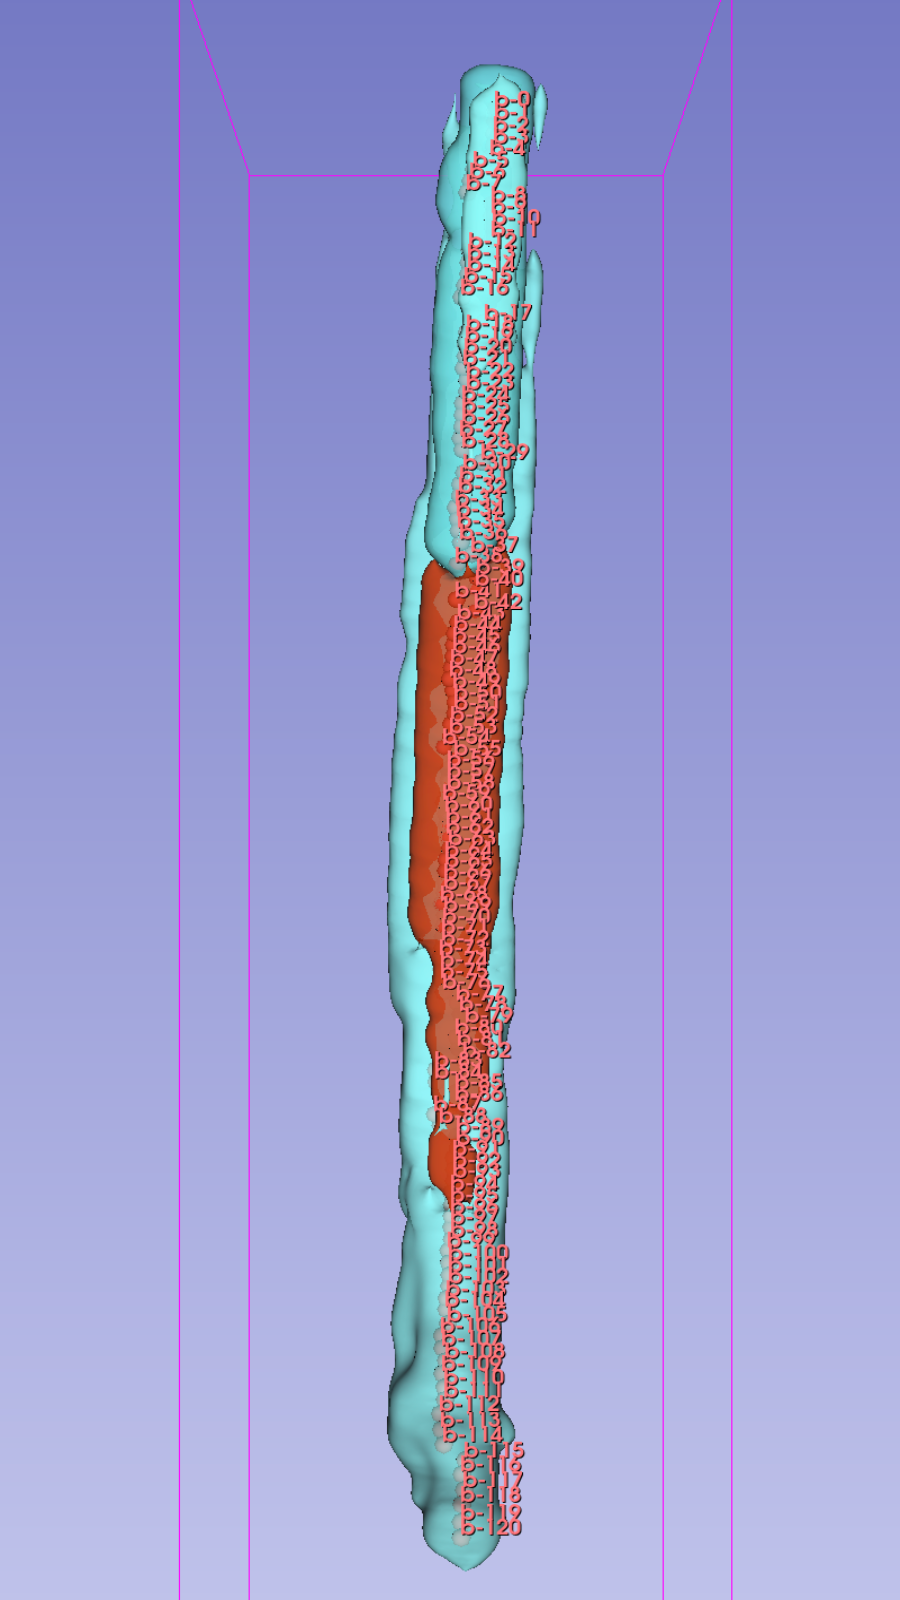
\includegraphics[width=\textwidth]{obrazy/spinal_canal_points_not_gap.png}
\caption{Punkty po całej wysokości}
\label{fig:scoliosis-spinal-canal-not-gap}
    \end{subfigure}
    \hfill
    \begin{subfigure}[b]{0.48\textwidth}
    \centering
    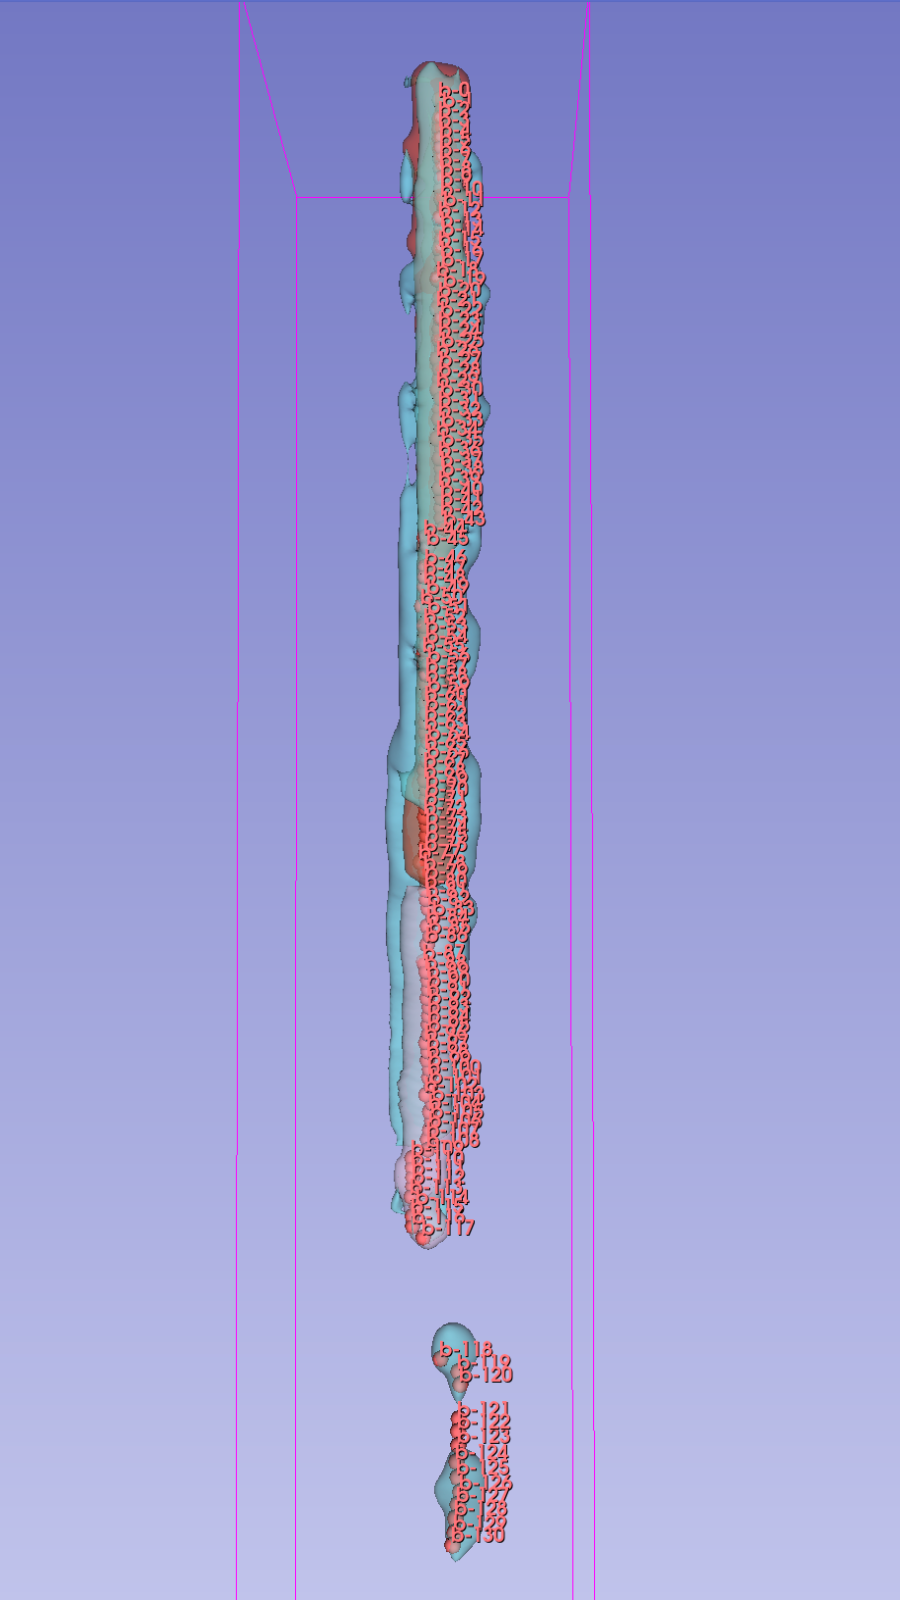
\includegraphics[width=\textwidth]{obrazy/spinal_canal_points_gap.png}
    \caption{Brakujący fragment}
    \label{fig:scoliosis-spinal-canal-gap}
    \end{subfigure}
    \caption{Wyznaczone punkty kanału kręgowego przed uzupełnieniem brakujących fragmentów.}
\end{figure}

Algorytm odporny jest na brakujące fragmenty segmentacji, które mogą wyniknąć z lokalnie słabego sygnału danych wejściowych, artefaktów obrazowania lub błędu narzędzia segmentującego.
Aby umożliwić wyznaczenie ciągłej krzywizny kręgosłupa, niezbędnej do pomiaru kąta Cobba, zastosowano algorytm aproksymacji brakujących danych.
Zaimplementowana funkcja \texttt{approximate} realizuje zadanie uzupełniania brakujących danych przestrzennych (ubytków w segmentacji) przy wykorzystaniu interpolacji funkcjami sklejanymi trzeciego stopnia (ang. \textit{Cubic Spline Interpolation}).\cite{cubic-spline}

Przed przystąpieniem do aproksymacji kształtu kanału kręgowego, konieczna jest identyfikacja miejsc, w których proces segmentacji nie zwrócił wyników (tzw. luk w danych). W tym celu opracowano algorytm analizy dystrybucji punktów wzdłuż osi podłużnej (Z) kręgosłupa.

Niech $P = \{p_0, p_1, \dots, p_N\}$ będzie zbiorem uporządkowanych punktów (centroidów) wykrytych w procesie wstępnym. Algorytm iteruje przez pary sąsiednich punktów $(p_{i-1}, p_i)$, obliczając dystans wzdłuż osi Z:

\begin{equation}
    \Delta z_i = |z_i - z_{i-1}|
\end{equation}

Zdefiniowano parametry systemowe:
\begin{itemize}
    \item $h_{step}$ –- oczekiwany krok próbkowania, odpowiadający grubości warstwy badawczej (Slice Thickness) lub odstępowi między skanami (w implementacji przyjęto $h_{step} = 3.2$ mm).
    \item $T_{thresh}$ –- próg detekcji błędu, definiujący minimalną odległość uznawaną za lukę w danych.
\end{itemize}

Jeśli wyznaczona odległość $\Delta z_i$ przekracza próg $T_{thresh}$, algorytm klasyfikuje ten obszar jako ubytek segmentacji.
Liczba brakujących warstw $k_{miss}$ estymowana jest na podstawie ilorazu całkowitego odległości i oczekiwanego kroku:

\begin{equation}
    k_{miss} = \left\lfloor \frac{\Delta z_i}{h_{step}} \right\rfloor
\end{equation}

Na podstawie wartości $k_{miss}$, algorytm buduje dwie nowe przestrzenie indeksów:
\begin{enumerate}
    \item \textbf{Indeksy zachowane ($I_{rem}$):} odpowiadające punktom poprawnie wykrytym.
    \item \textbf{Indeksy brakujące ($I_{miss}$):} wirtualne znaczniki miejsc, które wymagają uzupełnienia.
\end{enumerate}

Ze względu na złożoną geometrię kręgosłupa w przestrzeni 3D, linia środkowa kanału kręgowego nie może być opisana jako prosta funkcja jednej zmiennej.
Zamiast tego zdefiniowano ją jako krzywą wektorową $\mathbf{C}(t)$, zależną od znormalizowanego parametru $t$:

\begin{equation}
    \mathbf{C}(t) = \begin{bmatrix}
                        x(t) \\ y(t) \\ z(t)
    \end{bmatrix}, \quad \text{dla} \quad t \in [0, 1]
\end{equation}
gdzie parametr $t$ reprezentuje znormalizowaną pozycję wzdłuż długiej osi kręgosłupa.
W implementacji parametr ten uzyskano poprzez liniowe mapowanie indeksów dostępnych warstw (\texttt{np.linspace}).

Problem interpolacji 3D rozłożono na trzy niezależne podproblemy jednowymiarowe.
Dla każdej współrzędnej przestrzennej ($\xi \in \{x, y, z\}$) skonstruowano funkcję sklejaną $S_\xi(t)$.
W każdym podprzedziale $[t_i, t_{i+1}]$ funkcja ta jest wielomianem trzeciego stopnia:

\begin{equation}
    S_\xi(t) = a_i + b_i(t - t_i) + c_i(t - t_i)^2 + d_i(t - t_i)^3
\end{equation}

Współczynniki $a_i, b_i, c_i, d_i$ wyznaczono tak, aby zapewnić ciągłość funkcji $S(t)$ oraz jej pierwszej $S'(t)$ i drugiej $S''(t)$ pochodnej w węzłach interpolacji.

W kodzie zastosowano naturalne warunki brzegowe (\texttt{bc\_type='natural'}), co jest kluczowe dla uniknięcia nienaturalnych wygięć krzywej na krańcach badanego odcinka.
Matematycznie oznacza to zerowanie się drugiej pochodnej (krzywizny) na końcach przedziału:

\begin{equation}
    S''_\xi(0) = 0 \quad \text{oraz} \quad S''_\xi(1) = 0
\end{equation}

Dla każdego brakującego fragmentu danych o indeksie $k_{miss}$, wyznaczono odpowiadającą mu wartość parametru $t_{miss}$ poprzez interpolację liniową znanych indeksów.
Ostateczne współrzędne punktu zrekonstruowanego $P_{rec}$ obliczono jako:

\begin{equation}
    P_{rec} = \left( S_x(t_{miss}), \; S_y(t_{miss}), \; S_z(t_{miss}) \right)
\end{equation}

Tak uzyskane punkty scalono z danymi oryginalnymi i posortowano, uzyskując ciągłą reprezentację geometryczną kanału kręgowego, co umożliwia dalsze precyzyjne pomiary kątów skrzywienia.

\begin{figure}[H]
    \centering
    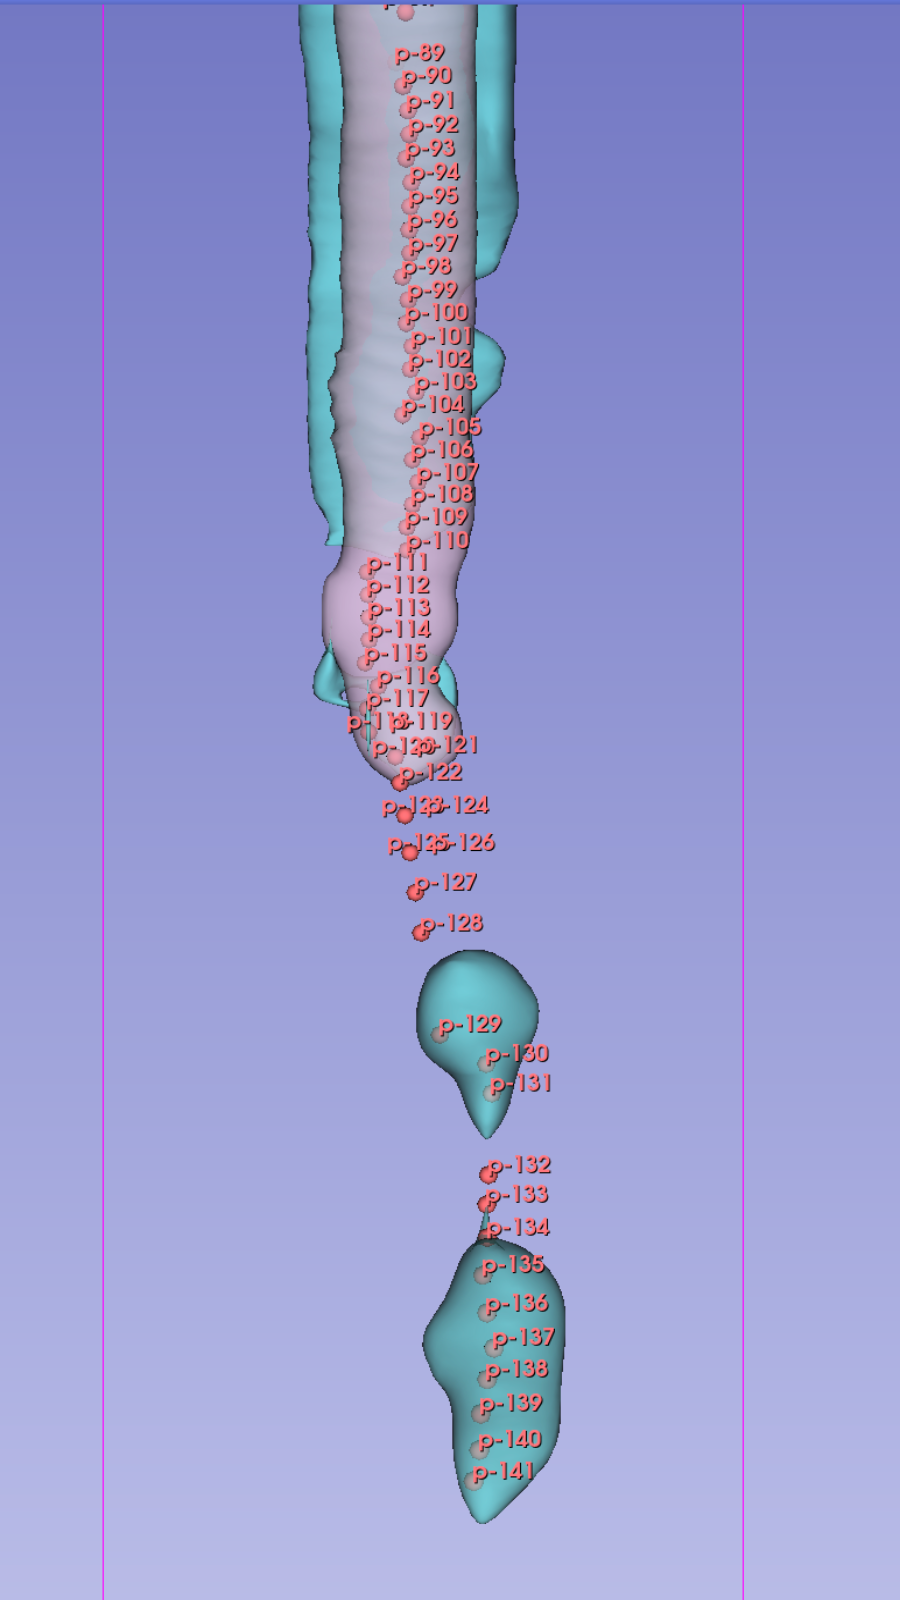
\includegraphics[width=0.5\textwidth]{obrazy/spinal_canal_filled_gaps.png}
    \captionsetup{justification=centering, font=small}
    \caption{Wypełnione luki segmentacji kanału kręgowego}
    \label{fig:scoliosis-filled-gaps}
\end{figure}

Po etapie rekonstrukcji ubytków, zbiór punktów reprezentujących kanał kręgowy posiada ciągłość, jednak dystrybucja punktów w przestrzeni może być niejednorodna.
Aby zapewnić stałą rozdzielczość przestrzenną niezbędną do precyzyjnych pomiarów geometrycznych, przeprowadzono proces reparametryzacji i zagęszczenia próbkowania.

Algorytm realizowany jest w trzech krokach:

W pierwszej kolejności usuwane są punkty, które dublują się lub znajdują się w odległości mniejszej niż błąd numeryczny ($\epsilon = 10^{-6}$).
Jest to krok niezbędny dla stabilności numerycznej algorytmów interpolacyjnych, które wymagają ściśle rosnącego argumentu funkcji.
\begin{equation}
    P_{filtered} = \{ p_i \in P : \| p_i - p_{i-1} \| > \epsilon \}
\end{equation}

W przeciwieństwie do poprzedniego etapu, gdzie parametrem była oś $Z$, tutaj zastosowano naturalną parametryzację krzywej w przestrzeni 3D.
Zdefiniowano parametr $s$, będący skumulowaną długością euklidesową wzdłuż łamanej łączącej kolejne punkty (ang. \textit{cumulative chord length}):

\begin{equation}
    s_0 = 0, \quad s_k = \sum_{i=1}^{k} \| p_i - p_{i-1} \|
\end{equation}

Dzięki temu dziedziną funkcji interpolującej staje się rzeczywista długość krzywej, a nie współrzędna kartezjańska, co pozwala na poprawne odwzorowanie pętli i silnych skrzywień niebędących funkcjami w sensie matematycznym względem jednej osi.

Na podstawie obliczonych odległości $s$, skonstruowano nowe funkcje sklejane trzeciego stopnia $C(s)$ dla każdej współrzędnej.
Następnie dokonano ponownego próbkowania (resampling) krzywej, generując nowy wektor parametrów $s'_{j}$ rozmieszczonych w idealnie równych odstępach:

\begin{equation}
    s'_{j} = j \cdot \frac{s_{max}}{M}, \quad \text{dla} \quad j = 0, \dots, M
\end{equation}
gdzie $M$ to nowa liczba próbek, ustalona jako dwukrotność liczby punktów wejściowych ($M = 2 \cdot N$).

W rezultacie uzyskano zbiór punktów $P_{new} = C(s')$, który charakteryzuje się:
\begin{itemize}
    \item \textbf{Większą gęstością:} dwukrotne zagęszczenie pozwala na precyzyjniejsze uchwycenie lokalnych zmian krzywizny.
    \item \textbf{Jednorodnością:} stały krok przestrzenny między punktami jest kluczowy dla algorytmów różniczkowych obliczających wektory styczne w kolejnych etapach analizy.
\end{itemize}

\begin{figure}[H]
    \centering
    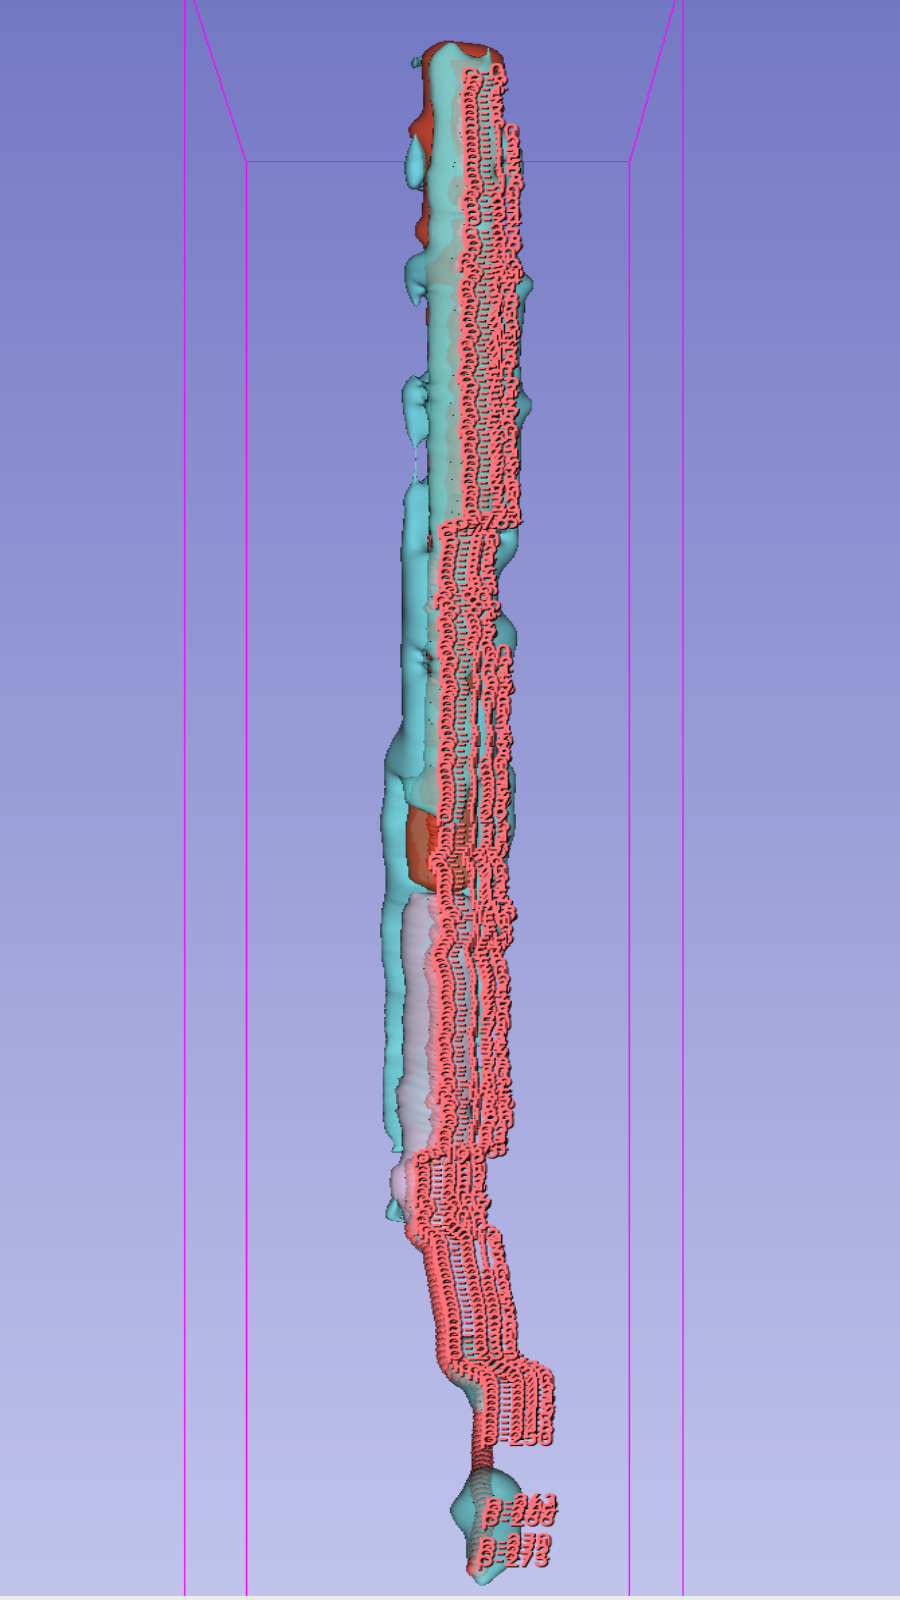
\includegraphics[width=0.5\textwidth]{obrazy/spinal-canal-equal-distribution.png}
    \captionsetup{justification=centering, font=small}
    \caption{Jednorodne zagęszczenie punktów kanału kręgowego}
    \label{fig:scoliosis-equal-distribution}
\end{figure}

\subsection{Wyznaczenie lokalnego układu współrzędnych kręgu}
\label{subsec:local-frame}

Po uzyskaniu kanału kręgowego z równomiernym rozmieszczeniem punktów następnym krokiem jest wyznaczenie lokalnego układu współrzędnych każdego kręgu w celu wyeliminowania błędów pomiarowych wynikających z naturalnej krzywizny kręgosłupa (lordozy lędźwiowej) oraz potencjalnej rotacji kręgów.

Pierwszym etapem analizy geometrycznej każdego kręgu jest wyznaczenie jego środka masy (centroidu).
Dla każdej odizolowanej etykiety kręgu $V$ obliczane są statystyki kształtu przy użyciu filtru \textit{LabelShapeStatisticsImageFilter}.
Centroid trzonu kręgu $C_{body}$ jest wyznaczany jako średnia arytmetyczna współrzędnych wszystkich wokseli należących do danej etykiety:
\begin{equation}
    \label{eq:centroid}
    C_{body} = \frac{1}{N} \sum_{i=1}^{N} P_i
\end{equation}
gdzie $P_{i}$ oznacza wektor współrzędnych $[x,y,z]^T$ $i$-tego woksela, należącego do kręgu, a $N$ jest całkowitą liczbą wokseli składających się na tę strukturę.

W celu wyznaczenia lokalnej orientacji, kręg musi zostać odniesiony do przebiegu kanału kręgowego.
Realizuje to funkcja \texttt{find\_closest\_i}, która przeszukuje zbiór punktów kanału $S=\{s_1,s_2,...,s_m\}$ wyznaczonych we wcześniejszym etapie szukając punktu o minimalnej odległości euklidesowej od centroidu kręgu:
\begin{equation}
    \label{eq:closest_point}
    i^* = \arg \min_{i \in \{1, \dots, m\}} \| \mathbf{s}_i - \mathbf{C}_{\text{body}} \|^2
\end{equation}
Zastosowanie kwadratu odległości pozwala na przyspieszenie obliczeń poprzez uniknięcie operacji pierwiastkowania, nie zmieniając przy tym położenia minimum funkcji.

Mając wyznaczony punkt odniesienia na kanale kręgowym, algorytm definiuje lokalne sąsiedztwo punktów (okno o rozmiarze 21 punktów), aby znaleźć lokalną krzywiznę.
Orientacja pionowa $y_{vec}$ jest wyznaczana przy użyciu analizy głównych składowych (ang. \textit{Principal Component Analysis} -- PCA)\cite{pca}, z pakietu \texttt{sklearn.decomposition}.
Dla lokalnego podzbioru punktów $S_{local}$ obliczana jest macierz kowariancji:
\begin{equation}
    \text{Cov}(S_{local}) = \frac{1}{n-1} \sum_{j=1}^{n} (s_j - \bar{s})(s_j - \bar{s})^T
\end{equation}
gdzie $\bar{s}$ jest wartością średnią pozycji punktów w oknie.
Wektor orientacji $y_{vec}$ odpowiada pierwszej składowej głównej (ang. \textit{principal component}), która wskazuje kierunek największej wariancji zbioru punktów, czyli w tym przypadku kierunek styczny do kanału kręgowego.
Wyznaczony wektor jest normalizowany do jedności:

\begin{equation}
    \label{eq:normalize_y}
    \hat{y}_{vec} = \frac{\vec{y}_{vec}}{| \vec{y}_{vec} |}
\end{equation}

Ostatnim krokiem jest zapewnienie spójności zwrotu wektora.
W medycznym układzie współrzędnych przyjęto konwencję, w której oś $Z$ rośnie w kierunku czaszkowym (Superior).
Algorytm sprawdza składową $z$ wektora i w razie potrzeby dokonuje jego inwersji, aby wektor zawsze wskazywał kierunek dolny (inferior), zgodnie z przyjętą konwencją przebiegu osi kręgosłupa:

\begin{equation}
    \vec{y} =
    \begin{cases}
        -\hat{y}_{vec} & \text{jeżeli } (\hat{y}_{vec} \cdot [0, 0, 1]^T) > 0 \\
        \hat{y}_{vec} & \text{w przeciwnym razie}
    \end{cases}
\end{equation}

\begin{figure}[H]
    \centering
    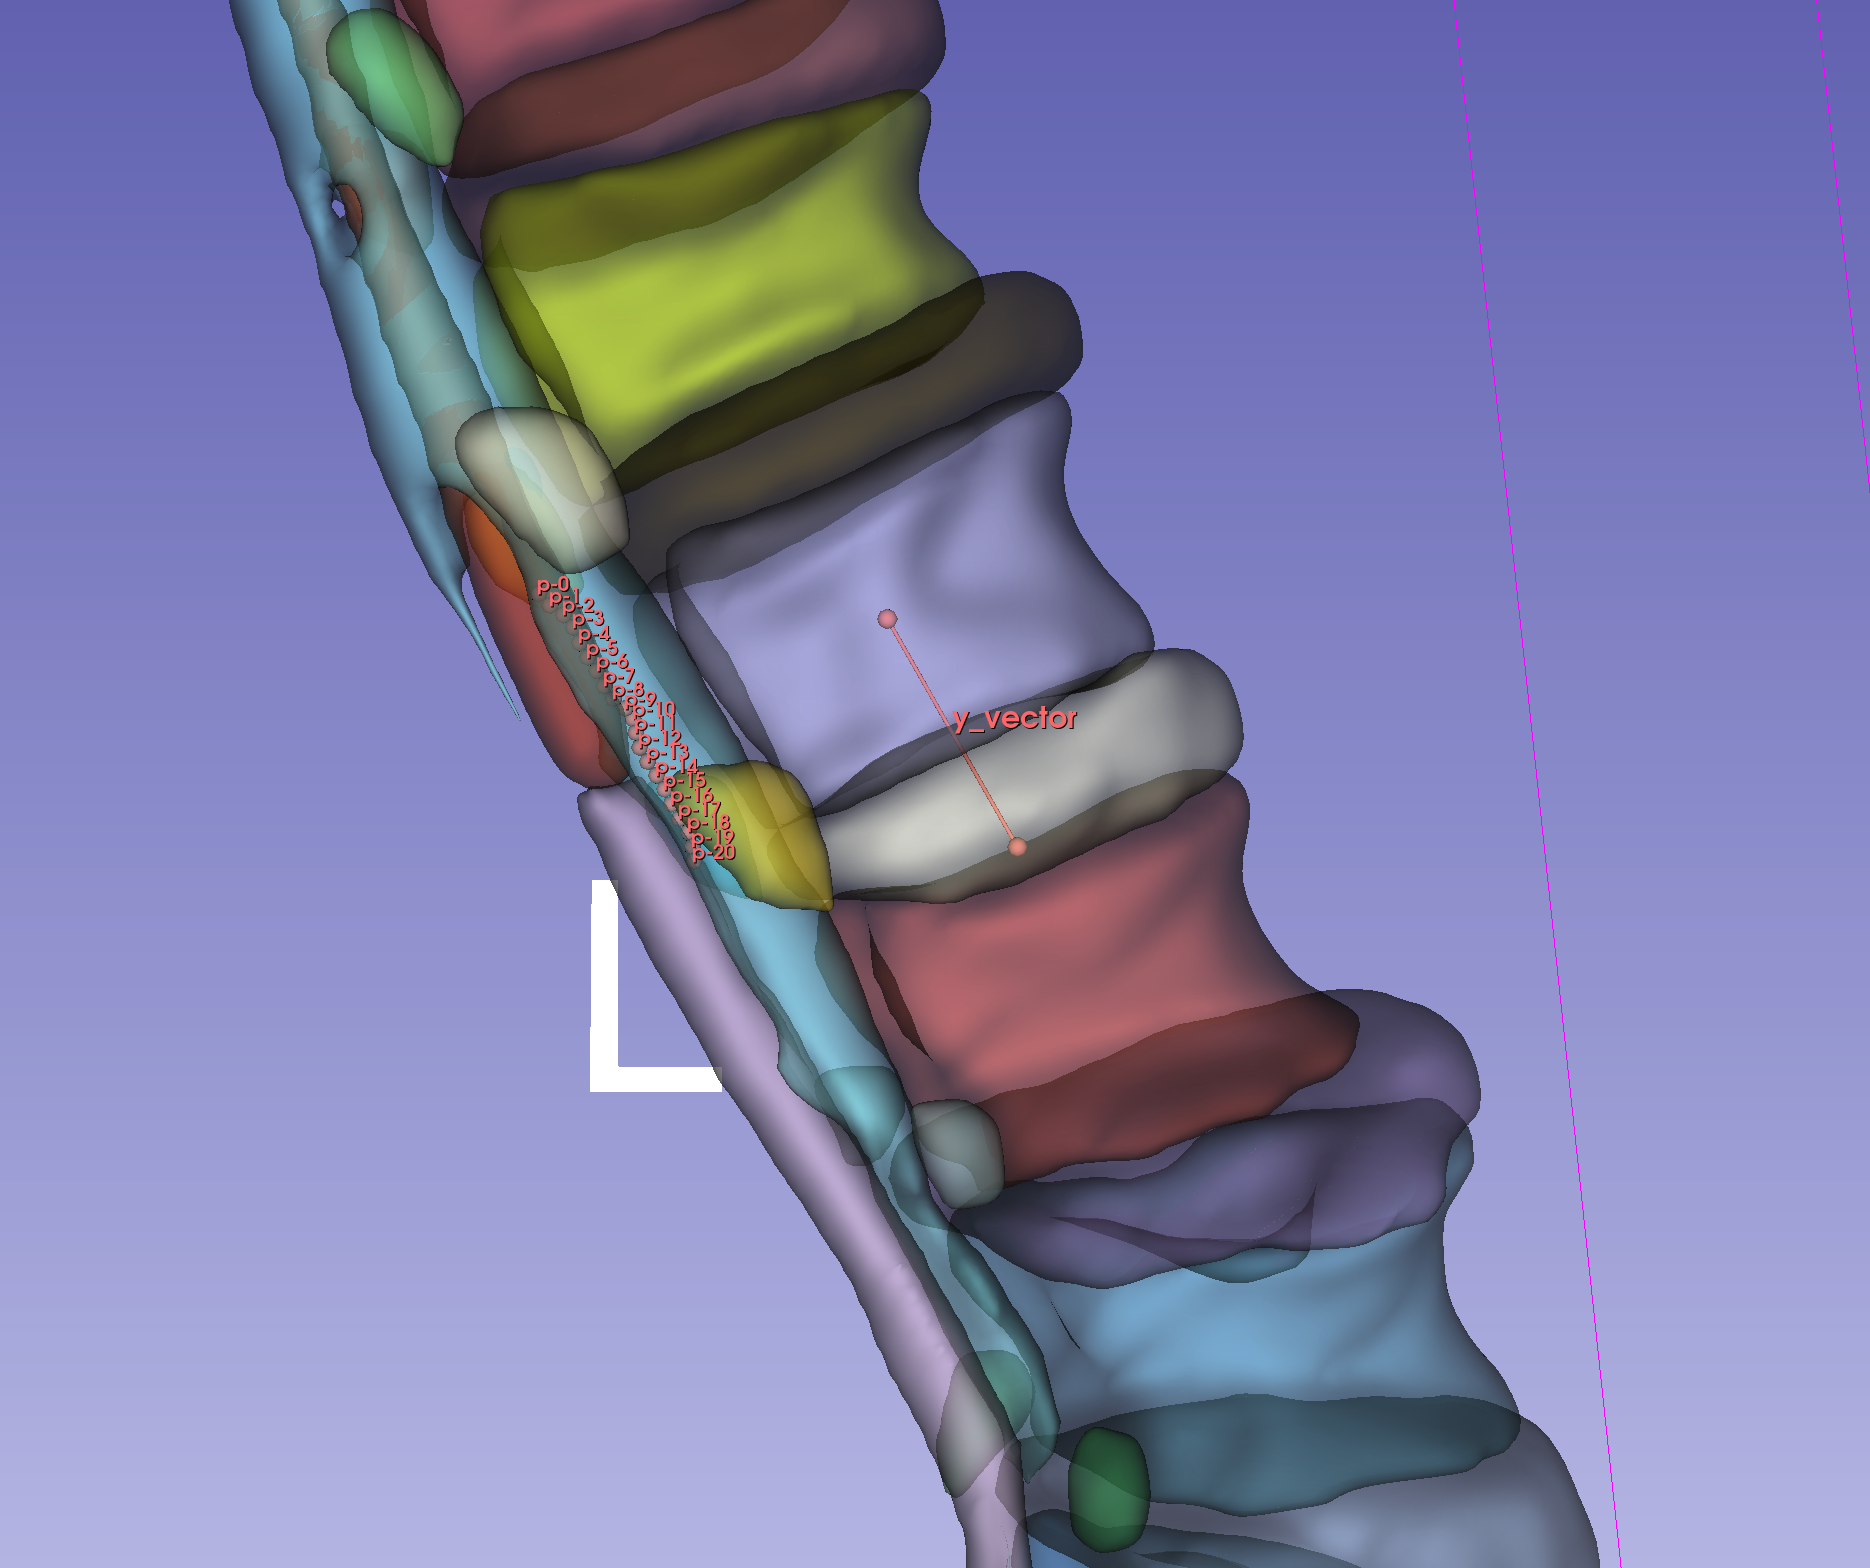
\includegraphics[width=0.75\textwidth]{obrazy/y_vec_with_points.png}
    \captionsetup{justification=centering, font=small}
    \caption{Wektor $\hat{y}_{final}$ dla jednego z kręgów (L2) wraz z lokalnymi punktami kanału kręgowego}
    \label{fig:v_vec_with_points}
\end{figure}

Po ustaleniu orientacji pionowej kręgu, algorytm przystępuje do wyznaczenia wektora $z$, który w lokalnym układzie współrzędnych reprezentuje oś przednio-tylną (\textit{anterior-posterior}).
Wektor $\vec{z}_{raw}$ jest definiowany jako różnica położeń między wcześniej obliczonym, w równaniu \eqref{eq:centroid}, centroidem trzonu kręgu $C_{body}$, a obliczonym w poprzedniej części algorytmu najbliższym punktem kanału kręgowego $\mathbf{s}_{i^*}$ \eqref{eq:closest_point}.

\begin{equation}
    \vec{z}_{raw} = \mathbf{s}_{i^*} - C_{body}
\end{equation}

Wyznaczony wektor podobnie jak w \eqref{eq:normalize_y} normalizowany jest do jedności:

\begin{equation}
    \label{eq:normalize_z}
    \vec{z} = \frac{\vec{z}_{raw}}{| \vec{z}_{raw} |}
\end{equation}

\begin{figure}[H]
    \centering
    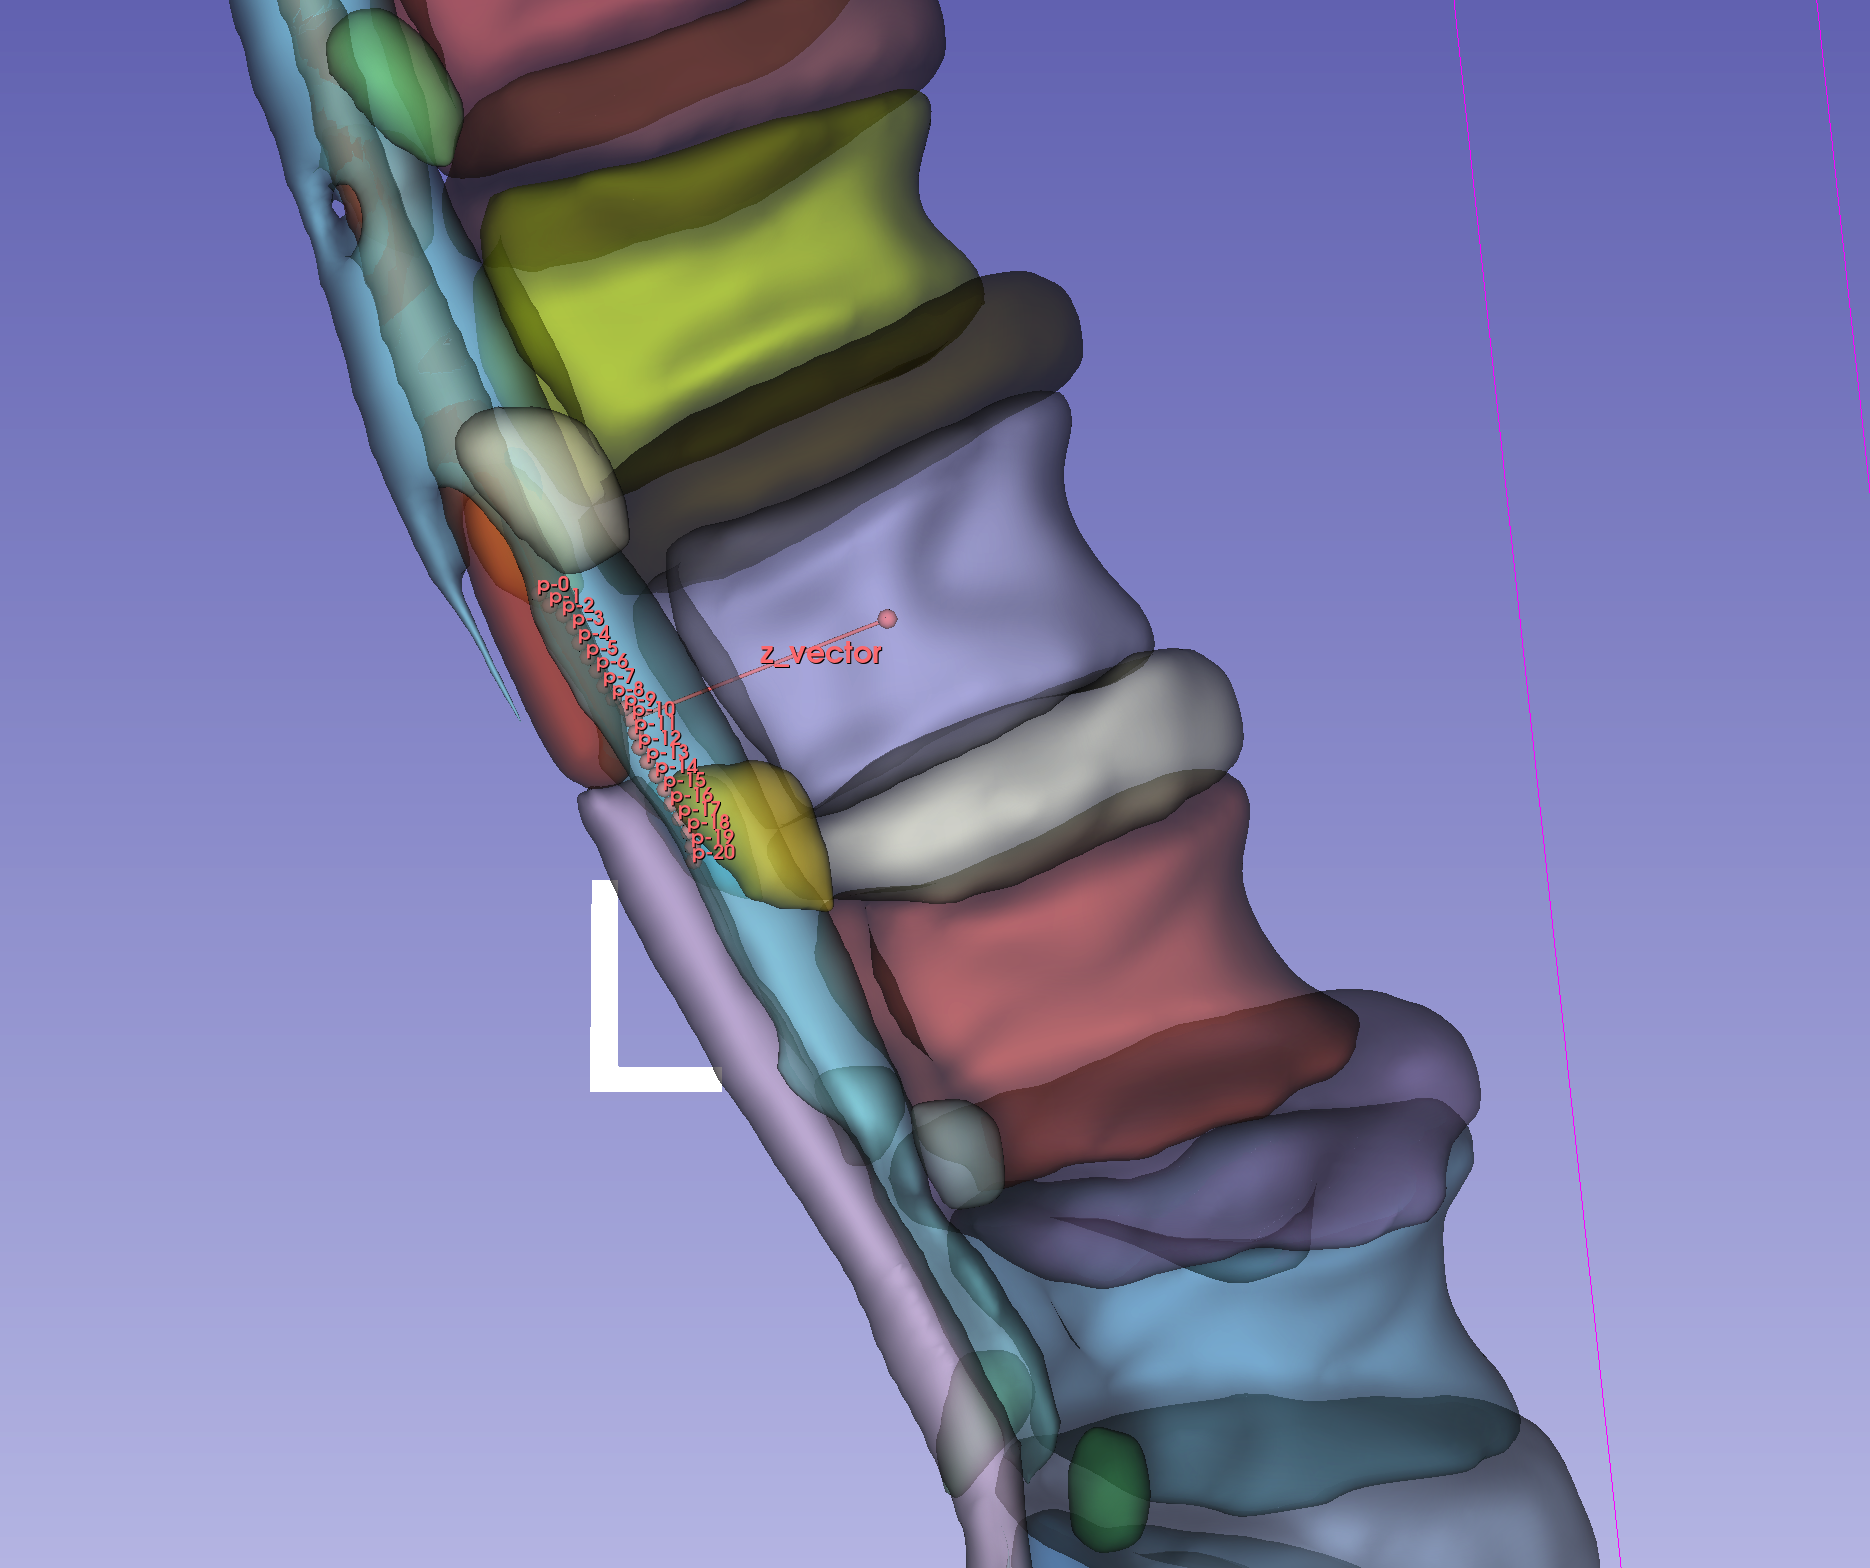
\includegraphics[width=0.75\textwidth]{obrazy/z_vec_with_points.png}
    \captionsetup{justification=centering, font=small}
    \caption{Wektor $\vec{z}$ dla jednego z kręgów (L2) wraz z lokalnymi punktami kanału kręgowego}
    \label{fig:z_vec_with_points}
\end{figure}

Ostatnim krokiem, mając wyznaczone dwa wektory jednostkowe $y$ (\eqref{eq:normalize_y}, styczny do kanału kręgowego w sąsiedztwie kręgu) oraz $z$ (\eqref{eq:normalize_z}, łączący środek trzonu z kanałem kręgowym), jest wyznaczenie trzeciego wektora $x$.
Wektor ten odpowiada osi boczno-przyśrodkowej (ang. \textit{medial-lateral}), czyli orientacji lewo-prawo.

Aby zapewnić idealną prostopadłość wszystkich osi, co jest niezbędne do poprawnego przepróbkowania obrazu bez wprowadzania deformacji geometrycznych, zastosowano operację iloczynu wektorowego.
Wektor $\vec{x}_{raw}$ jest wyznaczony jako iloczyn wektorowy osi grzbietowej oraz pionowej.

\begin{equation} \label{eq:cross_product_x} \vec{x}_{raw} = \vec{z} \times \vec{y}
\end{equation}

Zgodnie z definicją iloczynu wektorowego, wynikowy wektor $\vec{x}_{raw}$ jest prostopadły do obu wektorów wejściowych, co fizycznie odpowiada kierunkowi poprzecznemu względem płaszczyzny strzałkowej kręgu. Analogicznie jak w przypadku poprzednich osi, wektor $\vec{x}_{raw}$ zostaje poddany normalizacji, aby stał się wektorem jednostkowym.

\begin{equation} \label{eq:x_normalization} \vec{x} = \frac{\vec{x}_{raw}}{|\vec{x}_{raw}|}
\end{equation}

\begin{figure}[H]
    \centering
    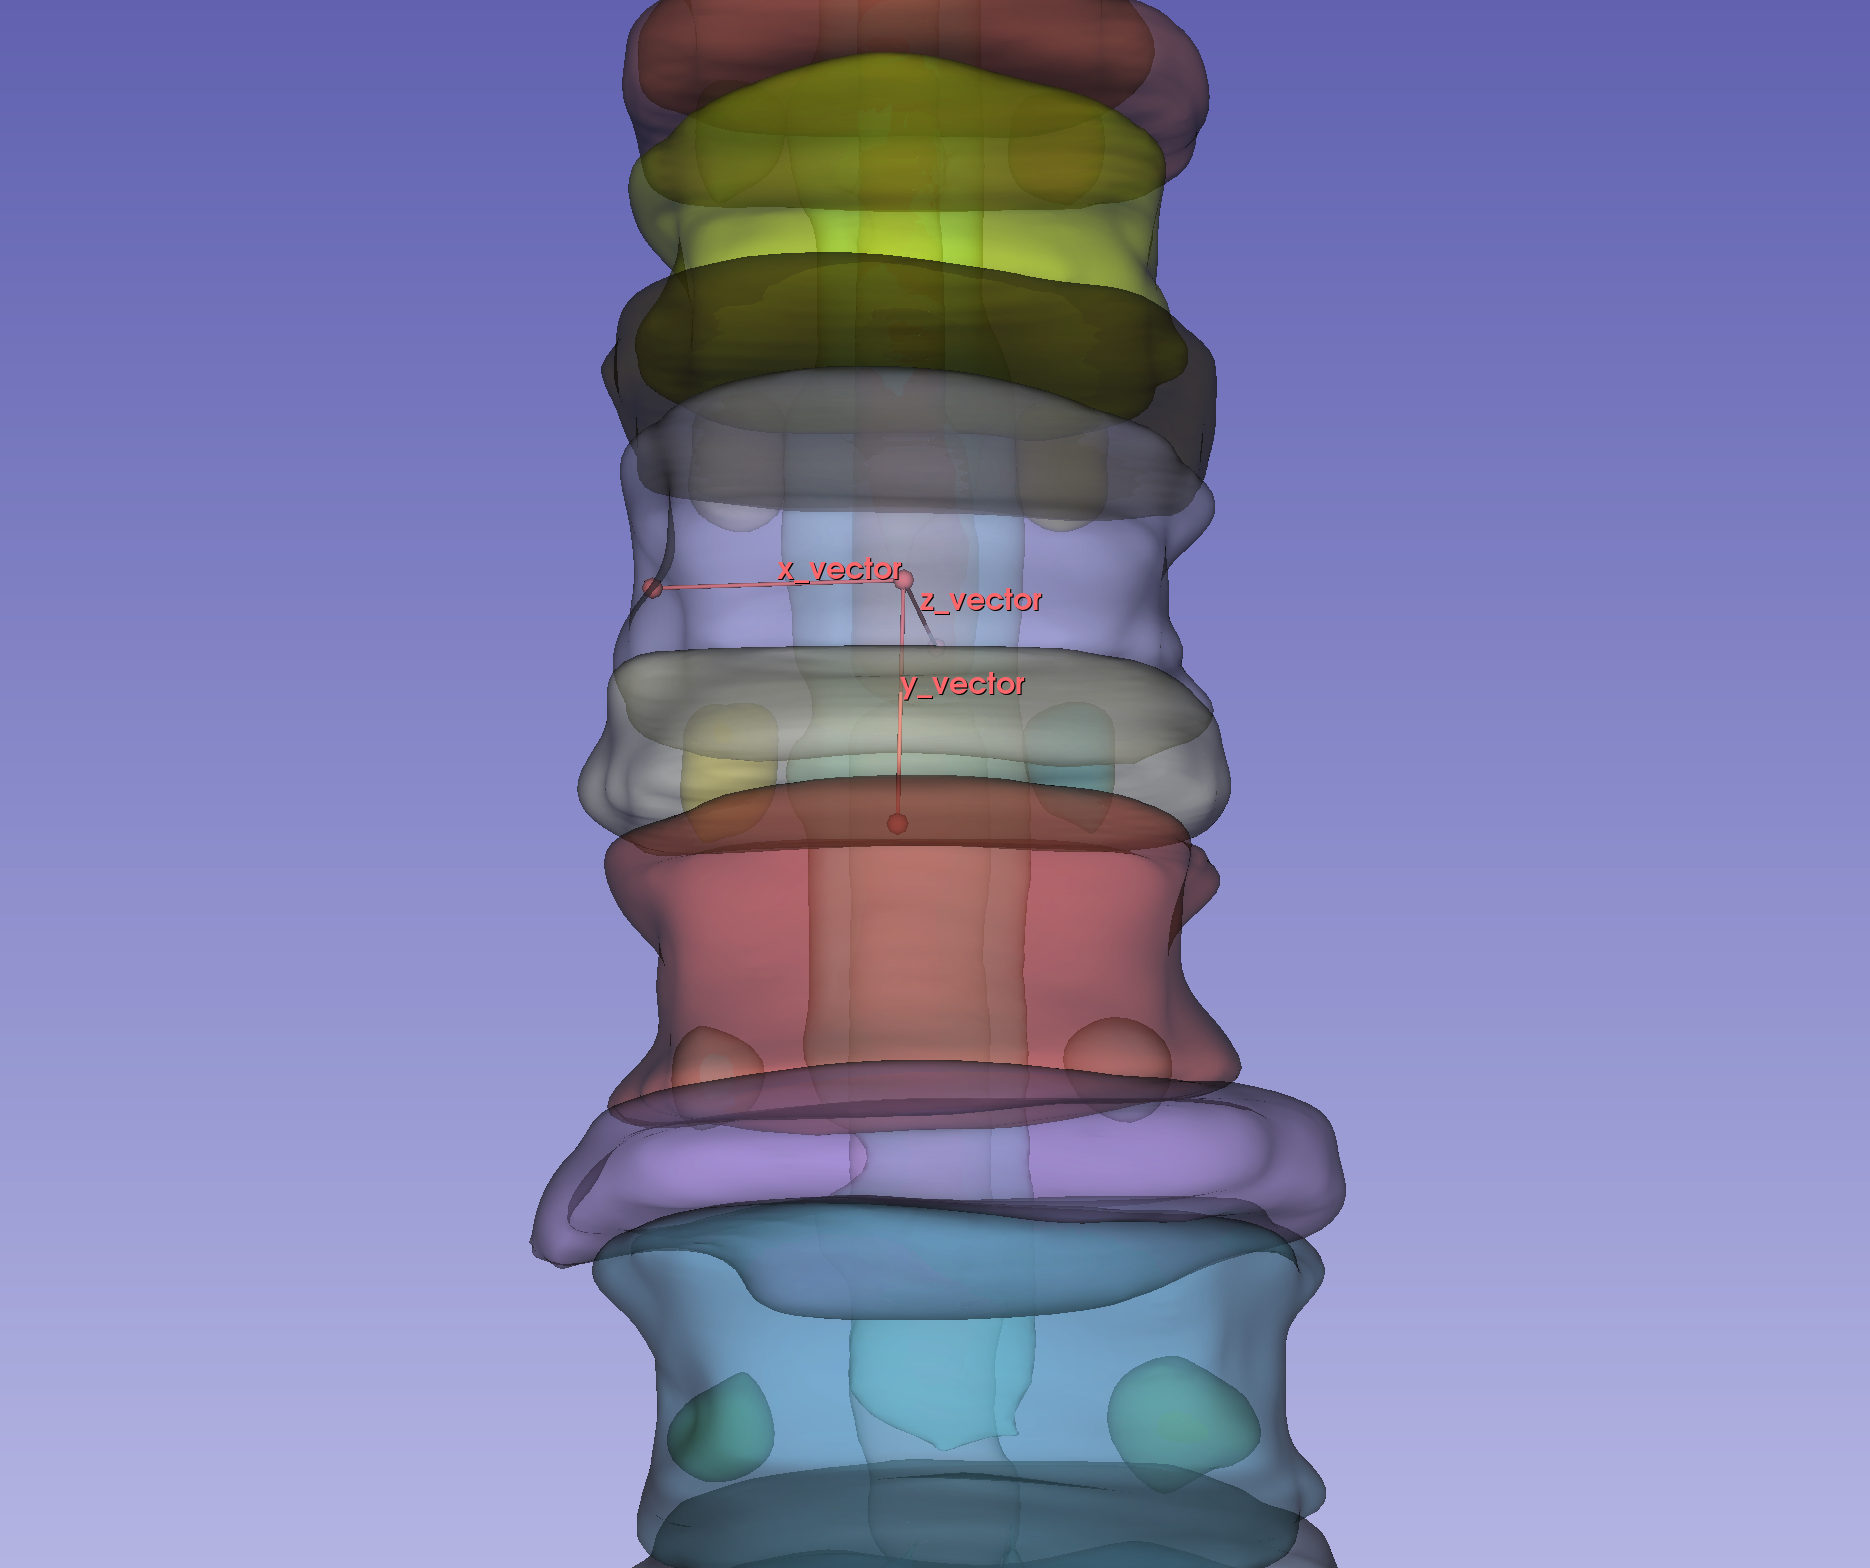
\includegraphics[width=0.75\textwidth]{obrazy/x_vec.png}
    \captionsetup{justification=centering, font=small}
    \caption{Wektor $\vec{x}$ dla jednego z kręgów (L2), wraz z pozostałymi wektorami tworzącymi lokalny układ współrzędnych.}
    \label{fig:x_vec}
\end{figure}


Po wyznaczeniu $\vec{x}$, w celu zagwarantowania dokładnej ortogonalności bazy, przeprowadzana jest re-ortogonalizacja wektora $\vec{z}$ jako iloczynu wektorowego $\vec{y}$ i $\vec{x}$:

\begin{equation} \label{eq:reorthogonalize_z}
    \vec{z} = \frac{\vec{y} \times \vec{x}}{|\vec{y} \times \vec{x}|}
\end{equation}

Krok ten eliminuje numeryczne błędy akumulowane podczas wyznaczania kolejnych wektorów bazy, zapewniając idealną ortogonalność układu $\{\vec{x}, \vec{y}, \vec{z}\}$.

\subsection{Ekstrakcja przekroju 2D i punktów narożnych trzonu}
\label{subsec:corner-points}

Wyznaczenie bazy ortonormalnej $\{\vec{x}, \vec{y}, \vec{z}\}$ pozwala na uniezależnienie procesu analizy od globalnego układu współrzędnych badania.
Następnym krokiem algorytmu jest wykorzystanie tej macierzy rotacji do przeprowadzenia operacji przepróbkowania (ang. \textit{resampling}).
Proces ten ma na celu przekształcenie trójwymiarowej chmury wokseli w serię zorientowanych diagnostycznie obrazów dwuwymiarowych.
Takie podejście pozwala na sprowadzenie złożonej geometrii przestrzennej kręgosłupa do płaszczyzny pomiarowej, na której możliwe jest zastosowanie klasycznych metod wizji komputerowej.

Przed przystąpieniem do przepróbkowania obrazu konieczne jest wyznaczenie fizycznego punktu początkowego nowej siatki obrazu (ang. \textit{origin}).
Punkt ten, oznaczony w algorytmie jako \texttt{anchor}, jest przesunięty względem centroidu kręgu $C_{body}$ tak, aby struktura trzonu w całości znalazła się w polu widzenia wynikowego obrazu o wymiarach \texttt{250×250} pikseli.

\begin{equation} \label{eq:anchor} P_{anchor} = C_{body} - 50\vec{x} - 50\vec{y}
\end{equation}
Przesunięcie o 50mm w kierunkach osi $\vec{x}$ i $\vec{y}$ pozycjonuje punkt początkowy tak, aby trzon kręgu znajdował się w polu widzenia algorytmu detekcji konturów.
Aby przekształcić dane z globalnej siatki wokseli do lokalnej płaszczyzny, konstruowana jest macierz kierunkowa (ang. \textit{Direction Matrix}) $\textbf{D}$.
Składa się ona z wektorów bazowych lokalnego układu współrzędnych.

\begin{equation} \label{eq:direction_matrix} \mathbf{D} = \begin{bmatrix}
                                                              x_0 & y_0 & z_0 \\ x_1 & y_1 & z_1 \\ x_2 & y_2 & z_2
\end{bmatrix}
\end{equation}
gdzie $[x_i, y_i, z_i]^T$ są składowymi znormalizowanych wektorów lokalnej bazy.

Właściwa ekstrakcja przekroju realizowana jest przy użyciu filtru \textit{ResampleImageFilter} z biblioteki SimpleITK.
Parametry wyjściowe obrazu zdefiniowano następująco:
\begin{itemize}
    \item \textbf{Rozmiar:} 250×250 pikseli.
    \item \textbf{Rozdzielczość (Spacing):} 0.5×0.5 mm na piksel, co pozwala na zachowanie wysokiej precyzji pomiarowej.
    \item \textbf{Interpolacja:} Metoda najbliższego sąsiada (\textit{Nearest Neighbor}).
\end{itemize}
Wybór interpolacji typu \textit{Nearest Neighbor} jest krytyczny, ponieważ przetwarzane dane wejściowe są mapą etykiet (segmentacją).
Zastosowanie interpolacji liniowej doprowadziłoby do powstania nieistniejących wartości pośrednich na granicach struktur, co uniemożliwiłoby poprawną detekcję krawędzi binarnych.
Dla każdego piksela (u,v) na wynikowym obrazie 2D, jego współrzędne w fizycznej przestrzeni 3D ($P_{phys}$) obliczane są zgodnie z przekształceniem afinicznym:

\begin{equation} \label{eq:resampling_math}
    P_{phys} = P_{anchor} + \mathbf{D} \cdot \begin{bmatrix} u \cdot s_u \\ v \cdot s_v \\ 0 \end{bmatrix}
\end{equation}

gdzie $s_u,s_v$ to wartości odstępu między pikselami (\textit{spacing}).
Wynikiem tej operacji jest obraz \texttt{resampled}, który stanowi bazę dla kolejnego etapu -- ekstrakcji konturu trzonu kręgu.

\begin{figure}[H]
    \centering
    \begin{subfigure}[b]{0.48\textwidth}
\centering
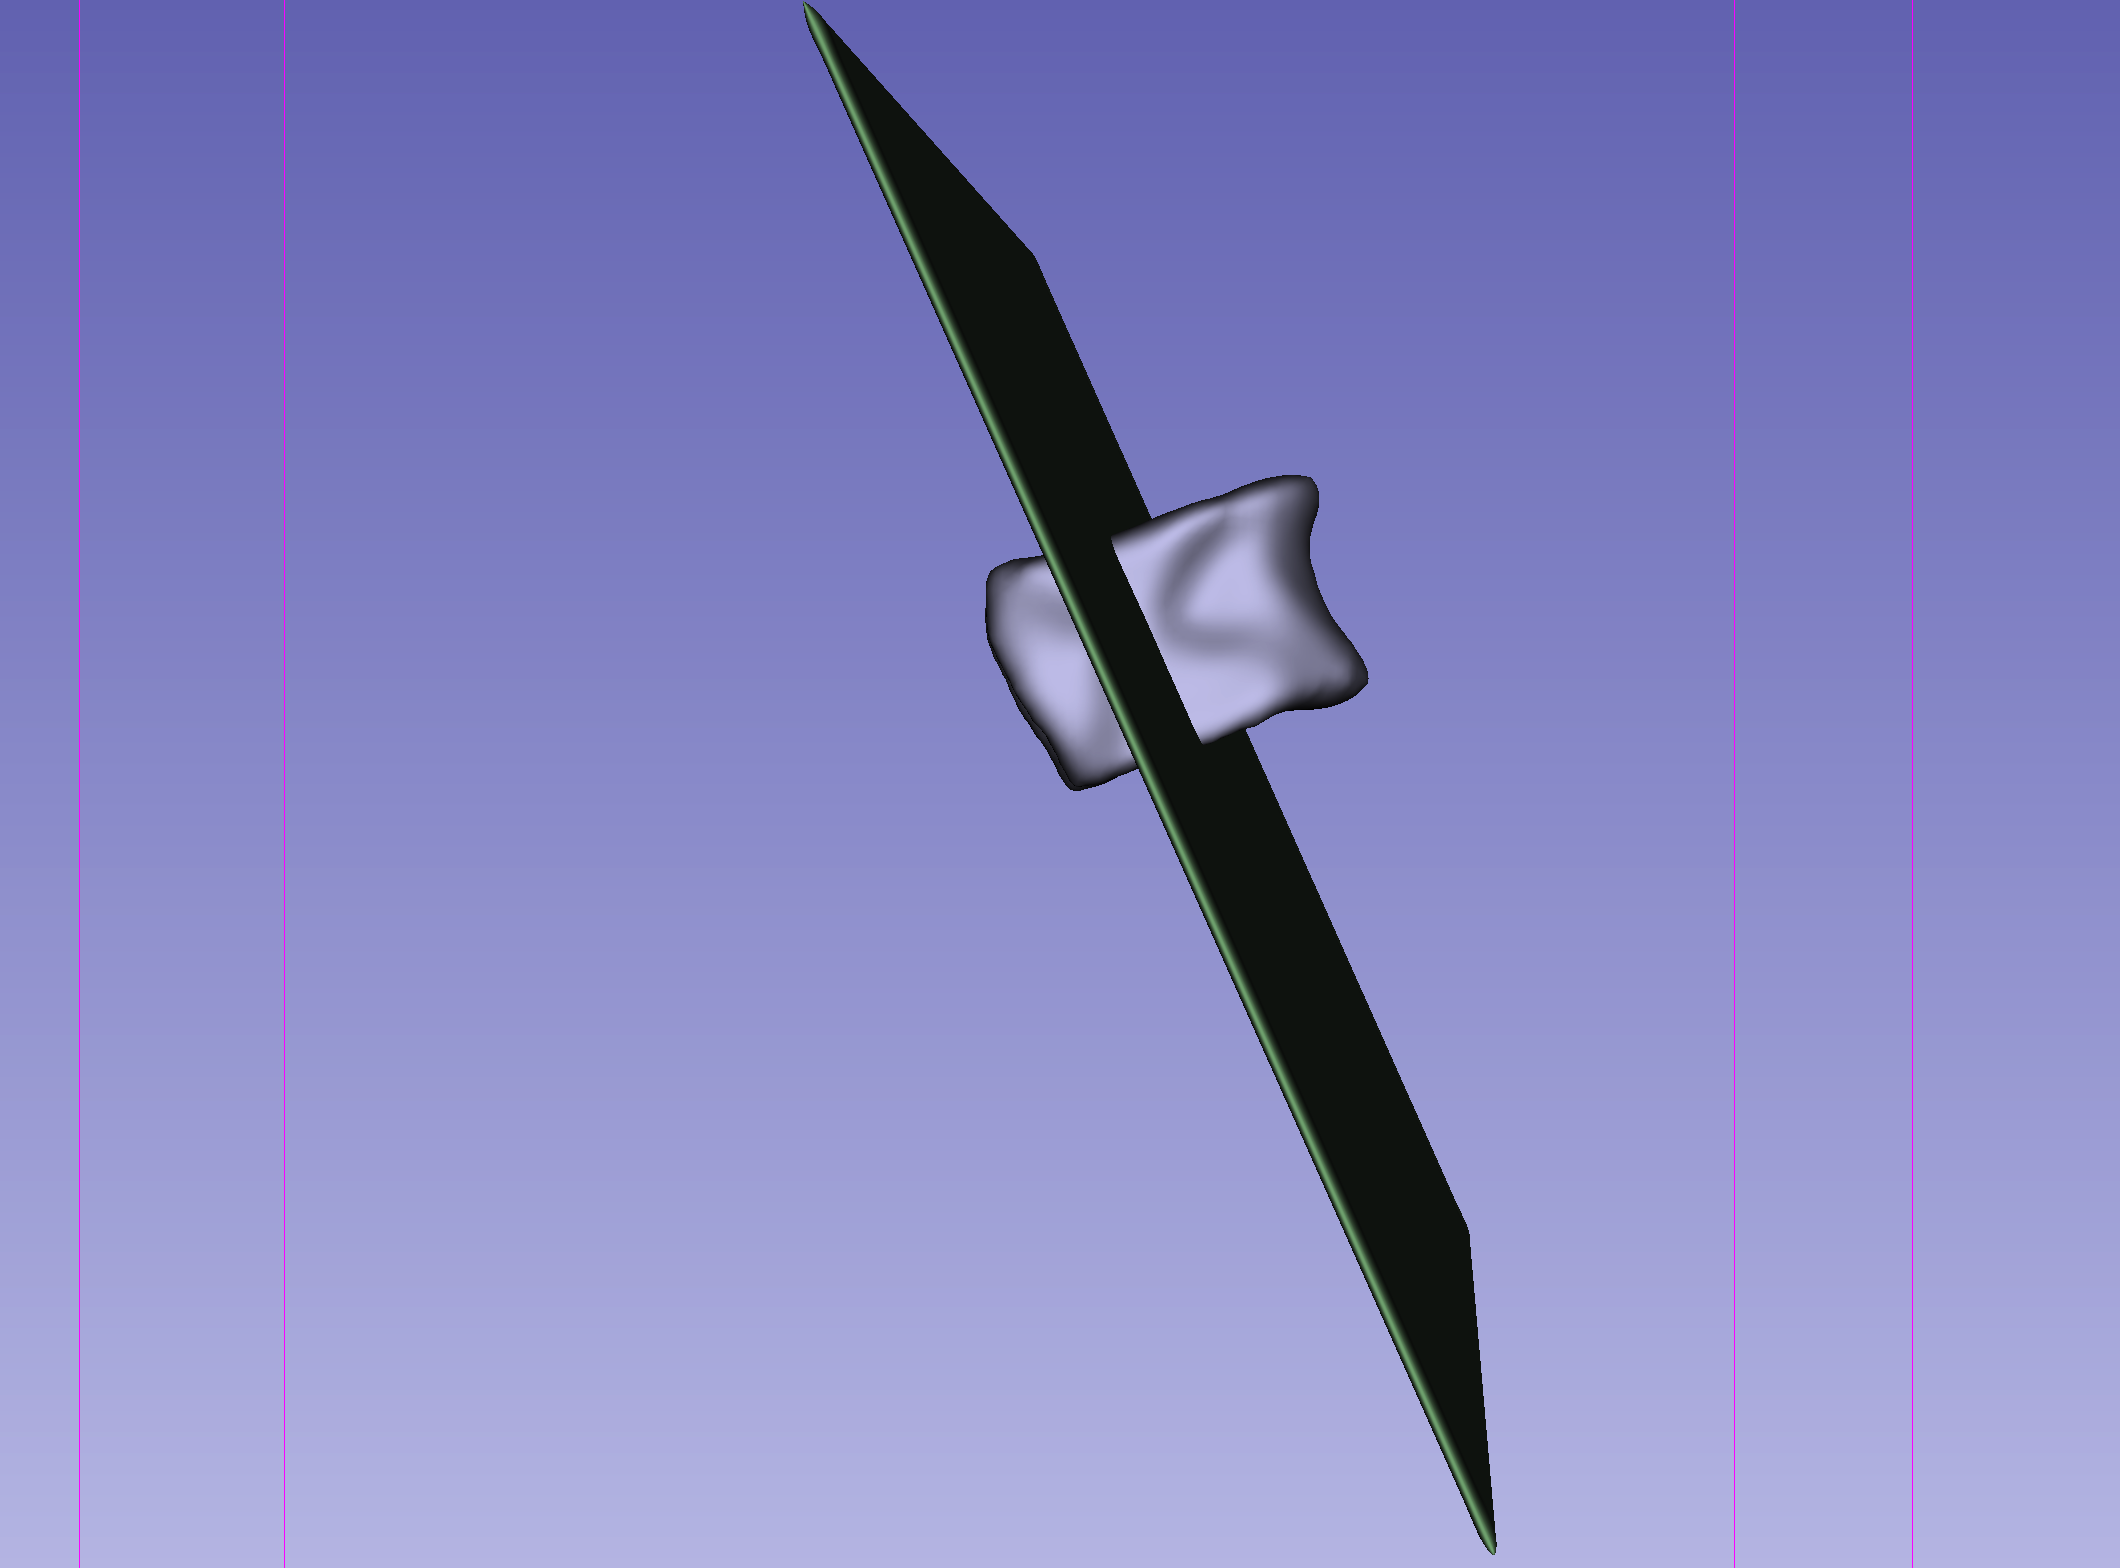
\includegraphics[width=\textwidth]{obrazy/left_plane.png}
\caption{Widok boczny badania}
\label{fig:scoliosis-left-plane}
    \end{subfigure}
    \hfill
    \begin{subfigure}[b]{0.48\textwidth}
    \centering
    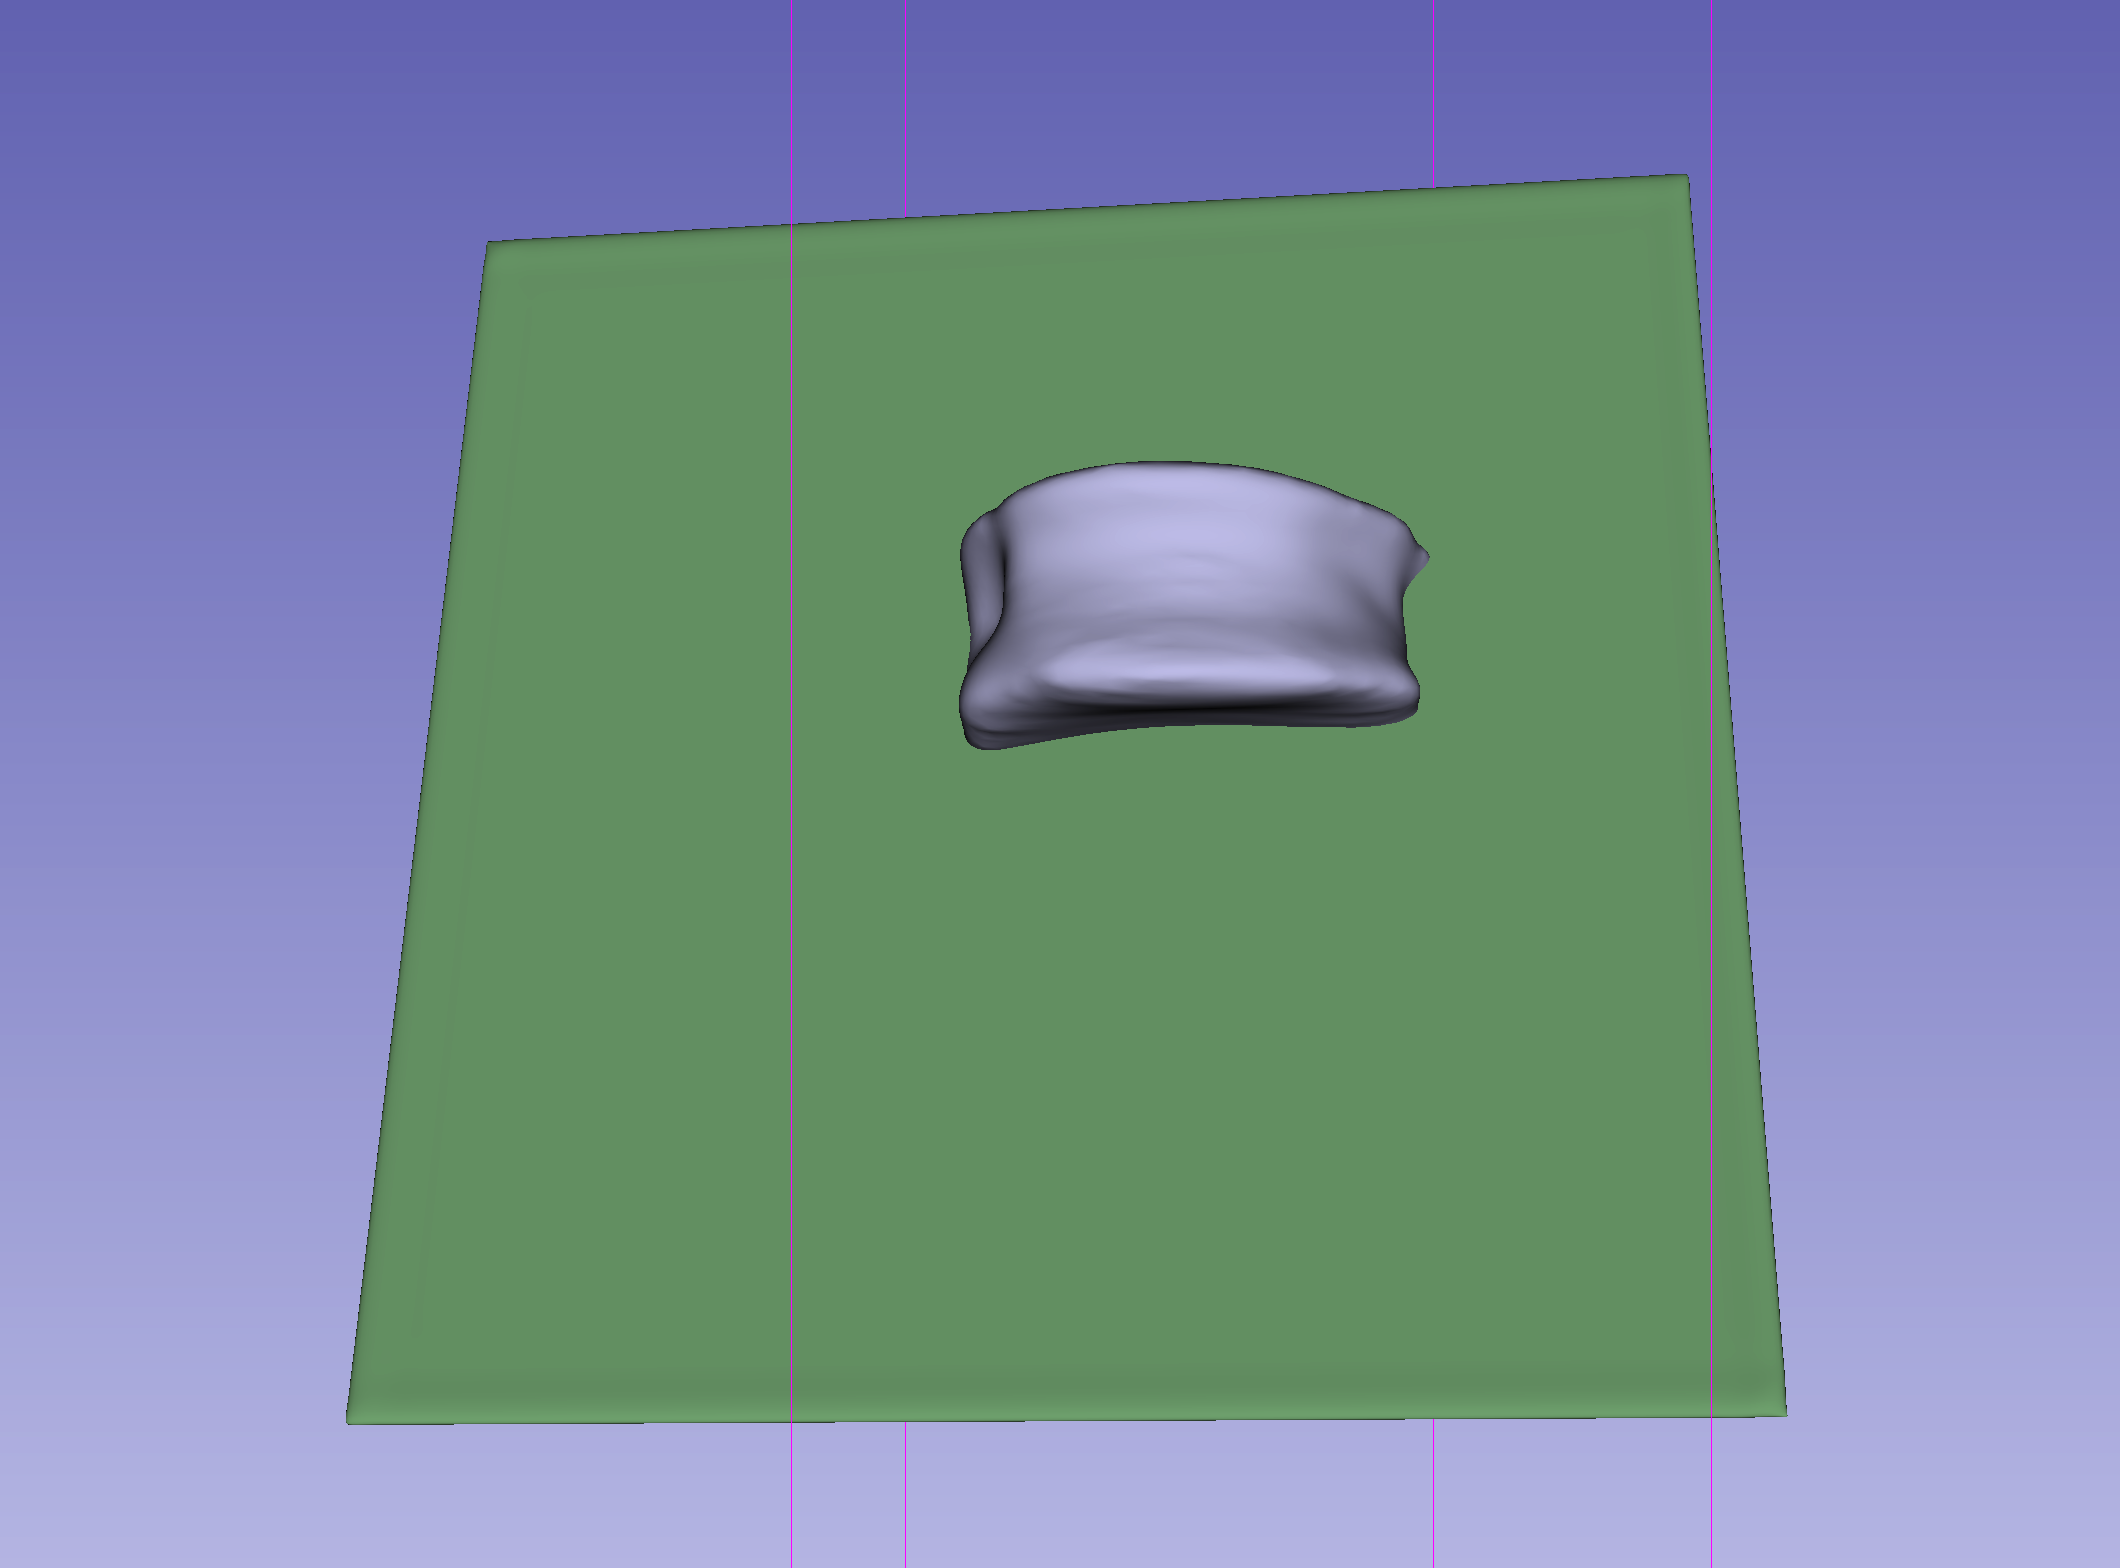
\includegraphics[width=\textwidth]{obrazy/anterior_plane.png}
    \caption{Widok czołowy badania}
    \label{fig:scoliosis-anterior-plane}
    \end{subfigure}
    \caption{Wizualizacja trójwymiarowa pojedynczego kręgu lędźwiowego wraz z nałożoną lokalną płaszczyzną przekroju strzałkowego, wyznaczoną na podstawie bazy ortonormalnej $\{\vec{x}, \vec{y}, \vec{z}\}$}
\end{figure}

\begin{figure}[H]
    \centering
    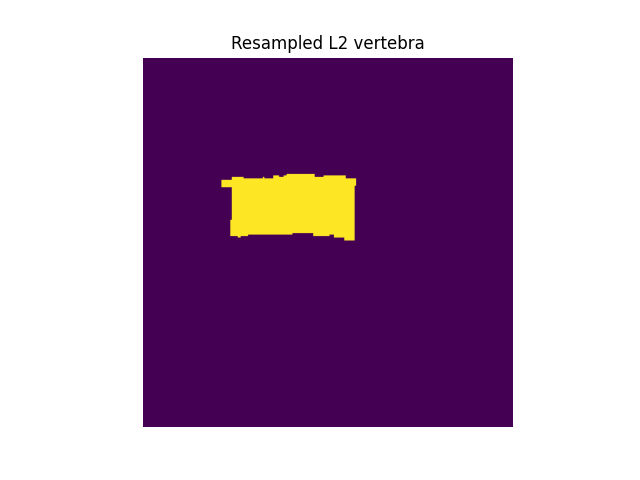
\includegraphics[width=0.75\textwidth]{obrazy/2d_resampled.png}
    \captionsetup{justification=centering, font=small}
    \caption{Wizualizacja dwuwymiarowa pojedynczego kręgu lędźwiowego na lokalnej płaszczyznie przekroju strzałkowego.}
    \label{fig:2d_resampled}
\end{figure}


Po uzyskaniu zorientowanego lokalnie przekroju 2D, algorytm przystępuje do kluczowego etapu analizy, którego celem jest wyznaczenie czterech punktów narożnych trzonu kręgu.
Punkty te definiują blaszki graniczne (górną i dolną), stanowiąc bezpośrednią podstawę do obliczenia kąta Cobba.
Do wyznaczenia tych struktur użyte będą metody z biblioteki OpenCV dla Pythona cv2\cite{opencv}.

W celu wyeliminowania drobnych artefaktów powstałych na etapie segmentacji, obraz poddawany jest operacji morfologicznego otwarcia (ang. \textit{morphological opening}, z biblioteki \texttt{cv2.morphologyEx(image, cv2.MORPH\_OPEN, np.ones((5, 5), np.uint8), iterations=2)})\cite{morph-opening}.
Wykorzystano element strukturalny o rozmiarze \texttt{5x5} pixeli co pozwala na wygładzenie brzegów struktury przy jednoczesnym zachowaniu jej pierwotnego kształtu oraz dwie iteracje, aby wyeliminować szum oraz drobne struktury niebędące częścią trzonu:
\begin{equation}
    I_{cleaned} = (I_{flat} \circ B)
\end{equation}
gdzie $B$ to kwadratowa macierz binarna, a symbol $\circ$ oznacza operację otwarcia.

Następnie, w celu precyzyjnego wyznaczenia granic trzonu, zastosowano detektor krawędzi Canny'ego\cite{canny} (z biblioteki \texttt{cv2.Canny(image, 0, 1)}, gdzie 0 i 1 to wartości graniczne dla obrazu binarnego trzonu kręgu i tła, między którymi wyznaczona będzie granica).
Pozwala on na zredukowanie informacji o całej masie kręgu do zbioru punktów brzegowych o szerokości jednego piksela.

Z wykrytych krawędzi ekstrahowany jest kontur zewnętrzny (z biblioteki \texttt{cv2.findContours(image, cv2.RETR\_EXTERNAL, cv2.CHAIN\_APPROX\_SIMPLE)}, z parametrami \texttt{RETR\_EXTERNAL} do wyznaczenia tylko zewnętrznych konturów oraz \texttt{CHAIN\_APPROX\_SIMPLE} do wykrycia tylko niezbędnych punktów).

Aby zniwelować wpływ lokalnych nierówności powierzchni trzonu kręgowego, algorytm wyznacza otoczkę wypukłą (ang. \textit{Convex Hull}) metodą z biblioteki \texttt{cv2.convexHull(contours)}.

Następnie zastosowano algorytm \textbf{Douglasa-Peuckera}\cite{douglas-peucker} (metoda \texttt{cv2.approxPolyDP(hull, arcLength * 0.01, True)} -- gdzie \texttt{arcLength * 0.01} to epsilon aproksymacji równy 1\% długości konturu; im mniejszy, tym bardziej wynikowy wielokąt przypomina oryginał, a trzeci parametr informuje, że krzywa ma być zamkniętą pętlą), który dokonuje aproksymacji wielokątowej konturu.
Proces ten redukuje liczbę punktów opisujących kształt, pozostawiając jedynie te najbardziej istotne z punktu widzenia geometrii struktury.

Ostatnim etapem analizy geometrycznej jest selekcja czterech kluczowych punktów narożnych z uzyskanego wielokąta aproksymacyjnego.
W tym celu zaimplementowano algorytm oparty na analizie sumy i różnicy współrzędnych $[x,y]$ punktów konturu, co pozwala na ich jednoznaczną klasyfikację topologiczną (lewy górny, prawy górny, lewy dolny, prawy dolny).
Metoda ta jest poprawna dla prostokątnych i quasi-prostokątnych kształtów (takich jak trzon kręgu).

Lewy górny róg ($P_{TL}$) oraz prawy dolny róg ($P_{BR}$) są identyfikowane poprzez minimalizację i maksymalizację sumy współrzędnych:
\begin{equation}
    P_{TL} = argmin(x_i + y_i), P_{BR} = argmax(x_i + y_i)
\end{equation}
Prawy górny róg ($P_{TR}$) oraz lewy dolny róg ($P_{BL}$) są wyznaczane poprzez analizę różnicy współrzędnych:
\begin{equation}
    P_{TR} = argmax(x_i - y_i), P_{BL} = argmin(x_i - y_i)
\end{equation}

\begin{figure}[H]
    \centering
    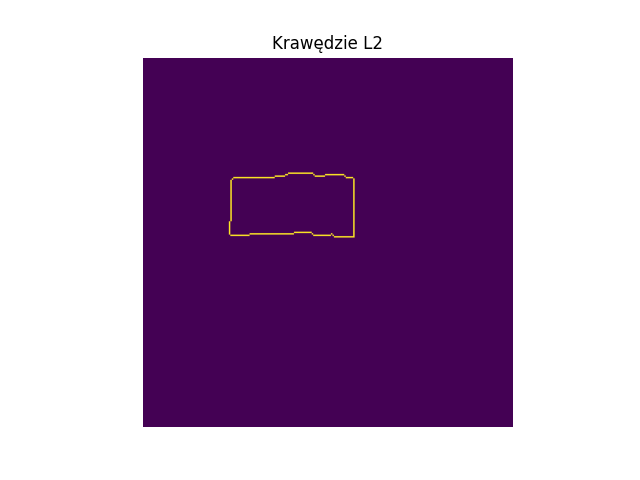
\includegraphics[width=1\textwidth]{obrazy/krawedzie_l2.png}
    \captionsetup{justification=centering, font=small}
    \caption{Wizualizacja wyznaczonej krawędzi pojedynczego kręgu lędźwiowego na lokalnej płaszczyznie przekroju strzałkowego.}
    \label{fig:edge}
\end{figure}

\begin{figure}[H]
    \centering
    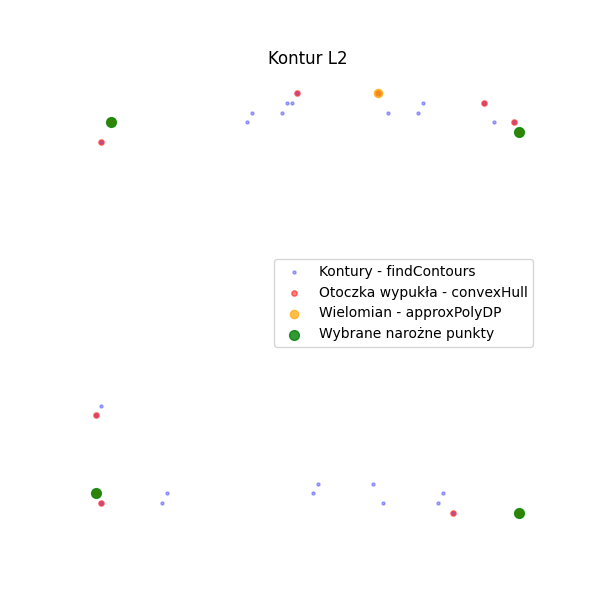
\includegraphics[width=1\textwidth]{obrazy/kontur_l2.png}
    \captionsetup{justification=centering, font=small}
    \caption{Wizualizacja etapów ekstrakcji cech geometrycznych trzonu.}
    \label{fig:contour}
\end{figure}

Wyznaczone punkty narożne reprezentują położenie struktur anatomicznych w układzie współrzędnych macierzy pikseli.
Ze względu na fakt, że analiza danych obrazowych wymaga uzyskania wyników o znaczeniu klinicznym, niezbędne jest przejście z jednostek bezwzględnych (pikseli) na jednostki fizyczne (milimetry).
Następnym etapem algorytmu jest zatem transformacja uzyskanych współrzędnych do trójwymiarowej przestrzeni lokalnego przekroju anatomicznego, zdefiniowanego we wcześniejszych etapach algorytmu:
\begin{equation}
    P_{\text{local,3D}} = \mathbf{T}_{\text{plane}} \cdot P_{\text{index}}
\end{equation}
gdzie $T_{plane}$ to macierz transformacji zdefiniowana dla zorientowanego lokalnie obrazu przekroju \eqref{eq:direction_matrix}.
Operacja ta, zaimplementowana jest jako \texttt{TransformContinuousIndexToPhysicalPoint} z biblioteki \texttt{SimpleITK}\cite{sitk}.
Dzięki temu uzyskane punkty $P_{start\_top}$, $P_{end\_top}$, $P_{start\_bot}$, $P_{end\_bot}$ posiadają współrzędne wyrażone w milimetrach, ale są one ściśle zablokowane na płaszczyźnie, która reprezentuję anatomię danego kręgu.

\begin{figure}[H]
    \centering
    \begin{subfigure}[b]{0.48\textwidth}
\centering
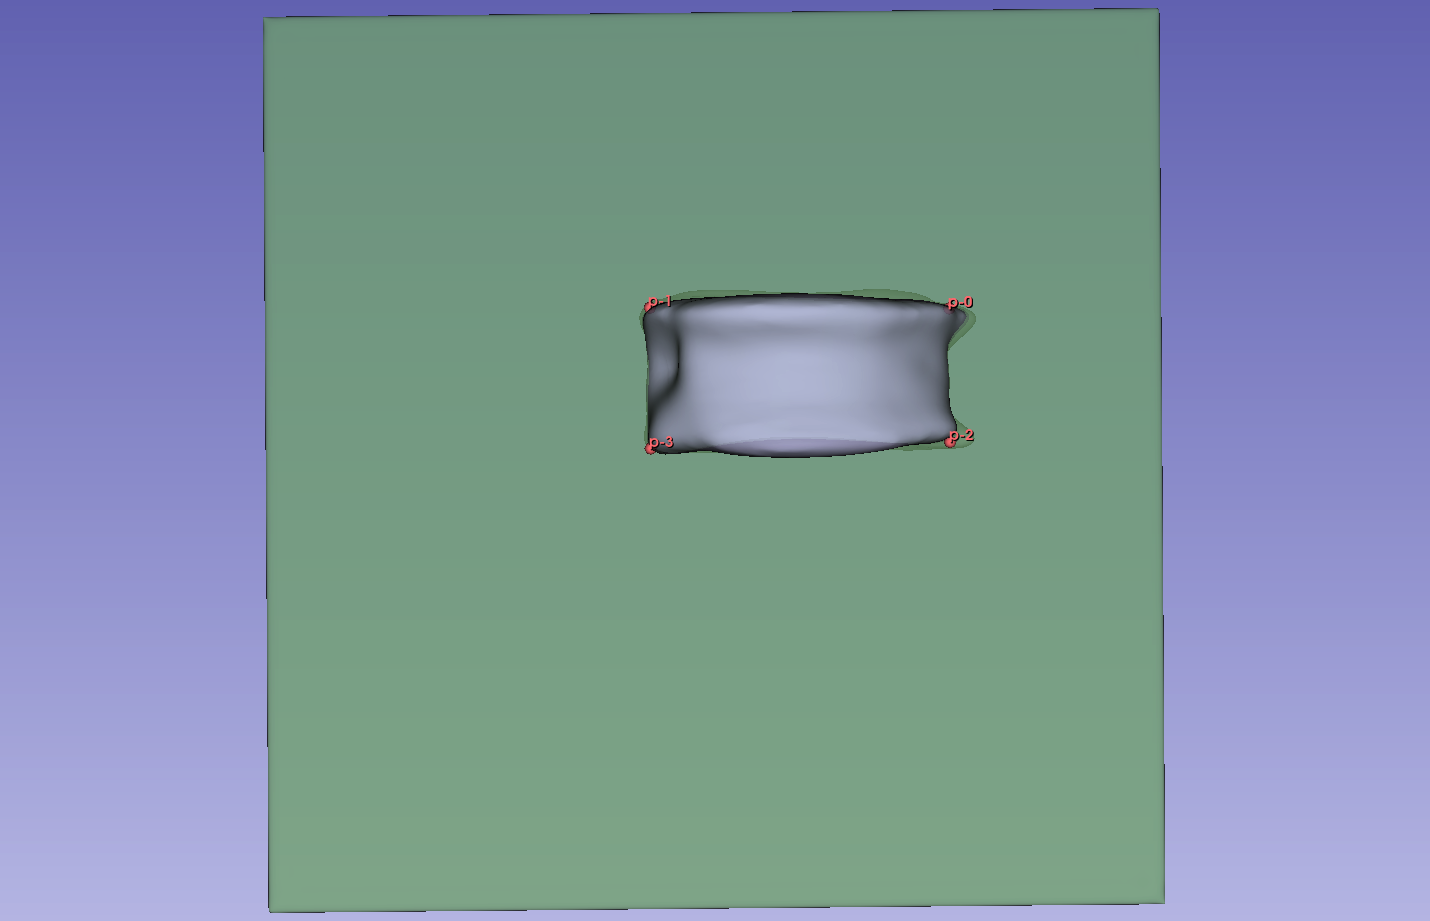
\includegraphics[width=\textwidth]{obrazy/anterior_contour.png}
\caption{Widok przedni}
\label{fig:anterior_contour}
    \end{subfigure}
    \hfill
    \begin{subfigure}[b]{0.48\textwidth}
    \centering
    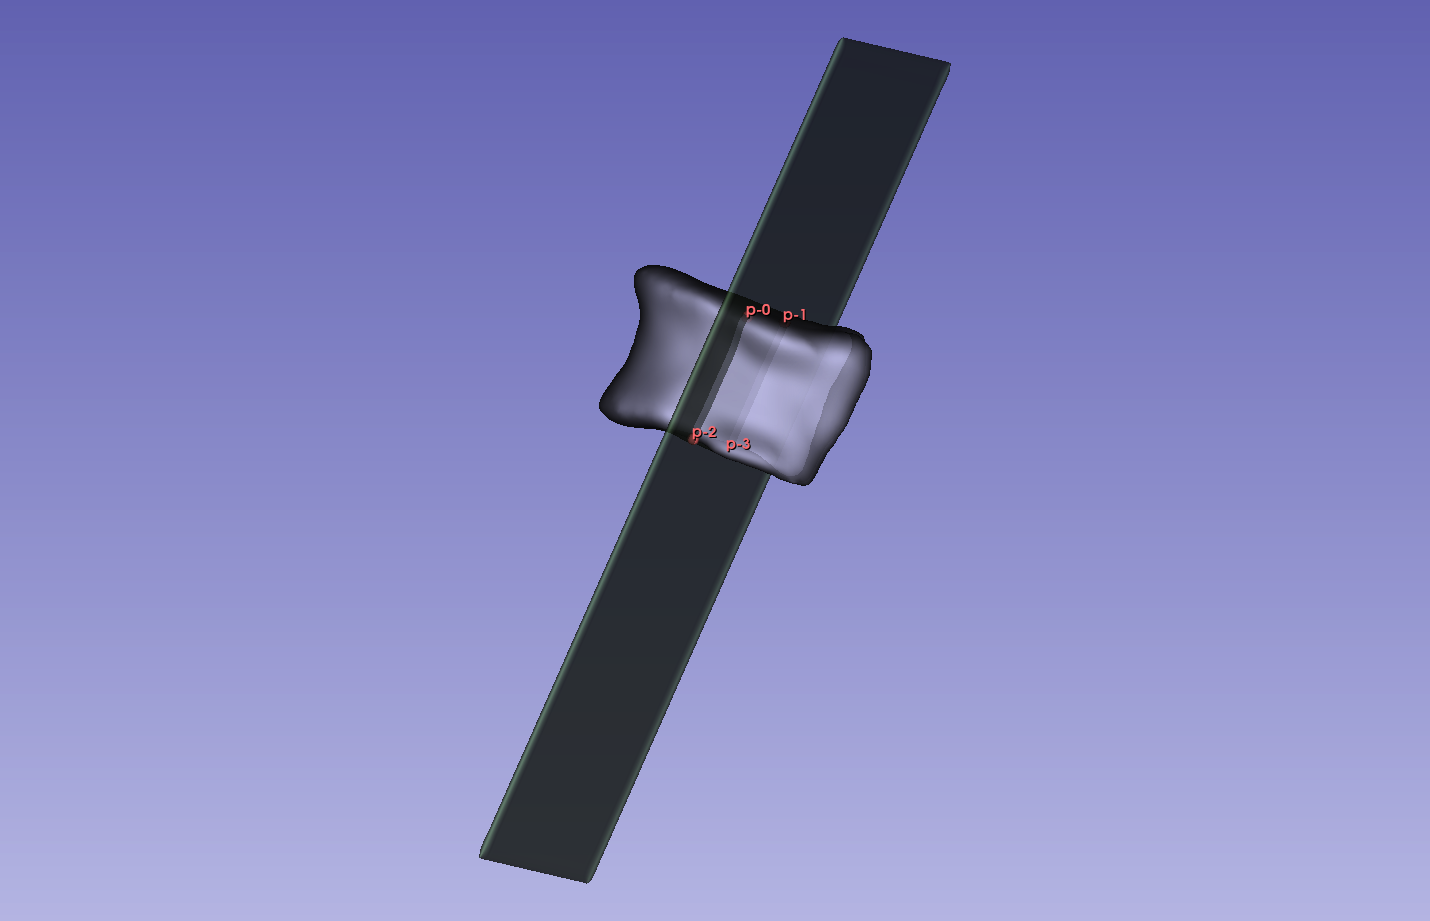
\includegraphics[width=\textwidth]{obrazy/left_contour.png}
    \caption{Widok boczny}
    \label{fig:left_contour}
    \end{subfigure}
    \caption{Przestrzenna wizualizacja wyników ekstrakcji punktów narożnych trzonu kręgu w lokalnym układzie współrzędnych płaszczyzny przekroju. Widoczne dopasowanie punktów do krawędzi struktury anatomicznej po transformacji z układu 2D do przestrzeni 3D.}
\end{figure}

\subsection{Pomiar kąta Cobba}
\label{subsec:cobb}
Po wyznaczeniu punktów narożnych dla każdego kręgu, algorytm przystępuje do finalnej fazy: wyznaczenia wspólnej płaszczyzny dla analizowanych par kręgów oraz obliczenia finalnej wartości kąta skrzywienia.
Ze względu na to, że kręgosłup w skoliozie ulega rotacji w trzech płaszczyznach, bezpośrednie rzutowanie punktów na standardowe płaszczyzny układu współrzędnych pacjenta (np. czołową) mogłoby prowadzić do niepoprawnego wyliczenia kąta.
Algorytm wykorzystuje metodę SVD (ang. \textit{Singular Value Decomposition}) do znalezienia płaszczyzny najlepiej dopasowanej do zbioru punktów narożnych analizowanej pary kręgów (górnego i dolnego).
Proces rozpoczyna się od wyznaczenia centroidu (środka geometrycznego) chmury punktów:
\begin{equation}
    \bar{p} = \frac{1}{n} \sum_{i=1}^{n} p_i
\end{equation}
Następnie dokonuje się centrowania danych poprzez odjęcie centroidu od każdego punktu:
\begin{equation}
    X_i = p_i - \bar{p}
\end{equation}
Zcentrowane punkty tworzą macierz $A \in \mathbb{R}^{n\times3}$.
Dekompozycja SVD macierzy $A$ zadana jest wzorem:
\begin{equation}
    A = U \Sigma V^T
\end{equation}
gdzie $V^T$ jest macierzą ortogonalną, której wiersze są wektorami własnymi macierzy kowariancji $A^{T}A$.
Wektor normalny $n$ szukanej płaszczyzny odpowiada wierszowi macierzy $V^T$, który jest związany z najmniejszą wartością osobliwą w macierzy $\Sigma$.
Wektor ten wskazuje kierunek, w którym wariancja danych jest najmniejsza, co matematycznie definiuje kierunek normalny do płaszczyzny najlepiej dopasowanej w sensie najmniejszych kwadratów odległości ortogonalnych.

Sama dekompozycja SVD dostarcza jedynie wektora normalnego $n$, prostopadłego do płaszczyzny pomiarowej.
Aby zdefiniować ortonormalną bazę $\{\vec{x}_{plane}, \vec{y}_{plane}\}$ rozpinającą tę płaszczyznę, wykorzystano dodatkowo kierunek przebiegu kręgosłupa $\vec{s}$, wyznaczony jako różnica środków geometrycznych chmur punktów narożnych kręgu górnego ($\bar{p}_{upper}$) i dolnego ($\bar{p}_{lower}$):
\begin{figure}[H]
    \centering
    \begin{subfigure}[b]{0.48\textwidth}
\centering
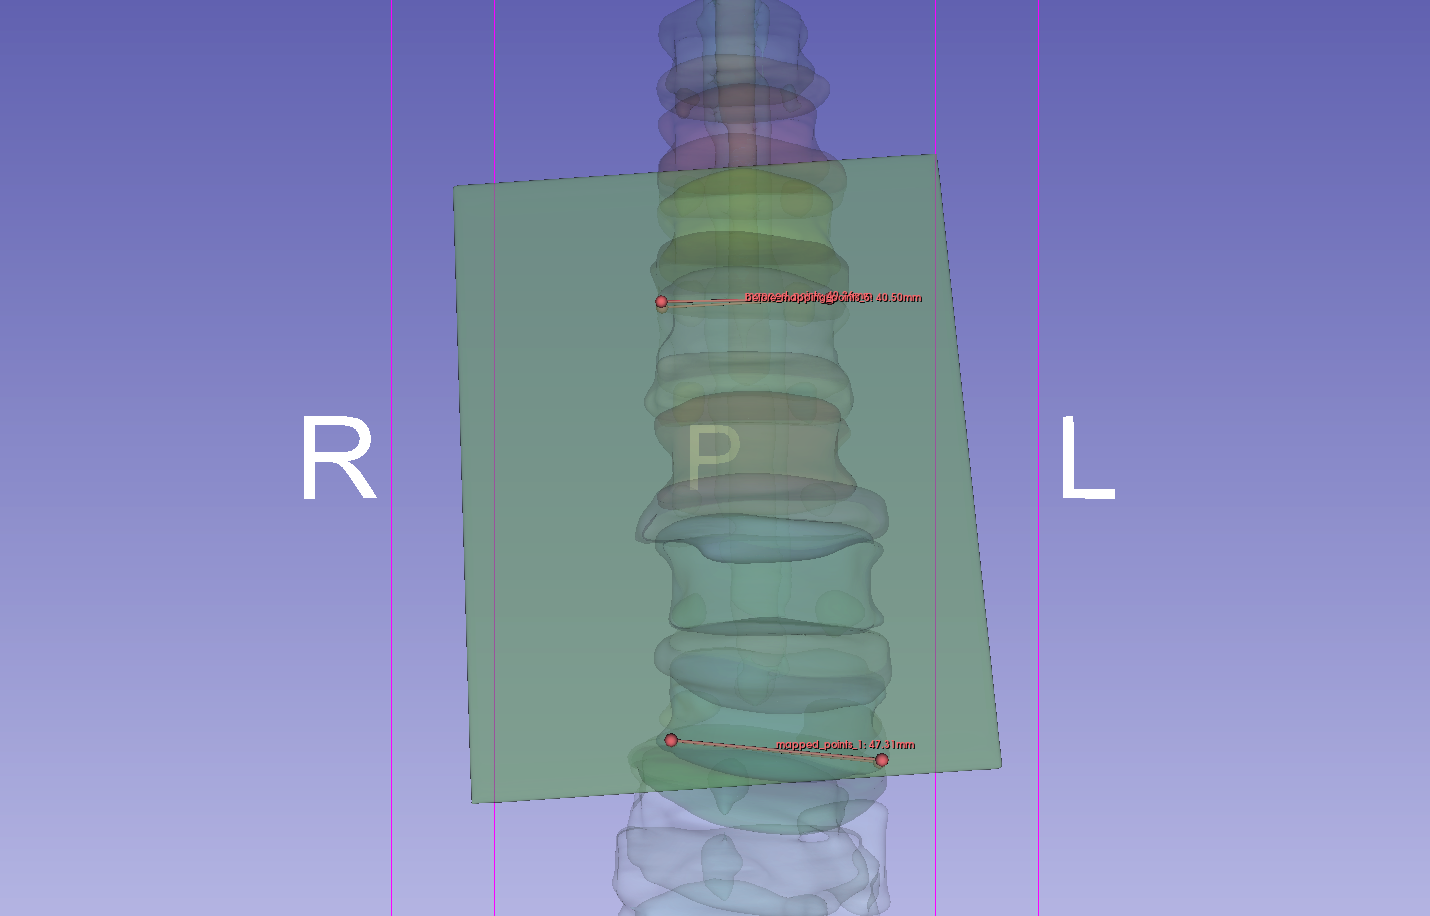
\includegraphics[width=\textwidth]{obrazy/common_plane_anterior.png}
\caption{Widok przedni}
\label{fig:anterior_plane}
    \end{subfigure}
    \hfill
    \begin{subfigure}[b]{0.48\textwidth}
    \centering
    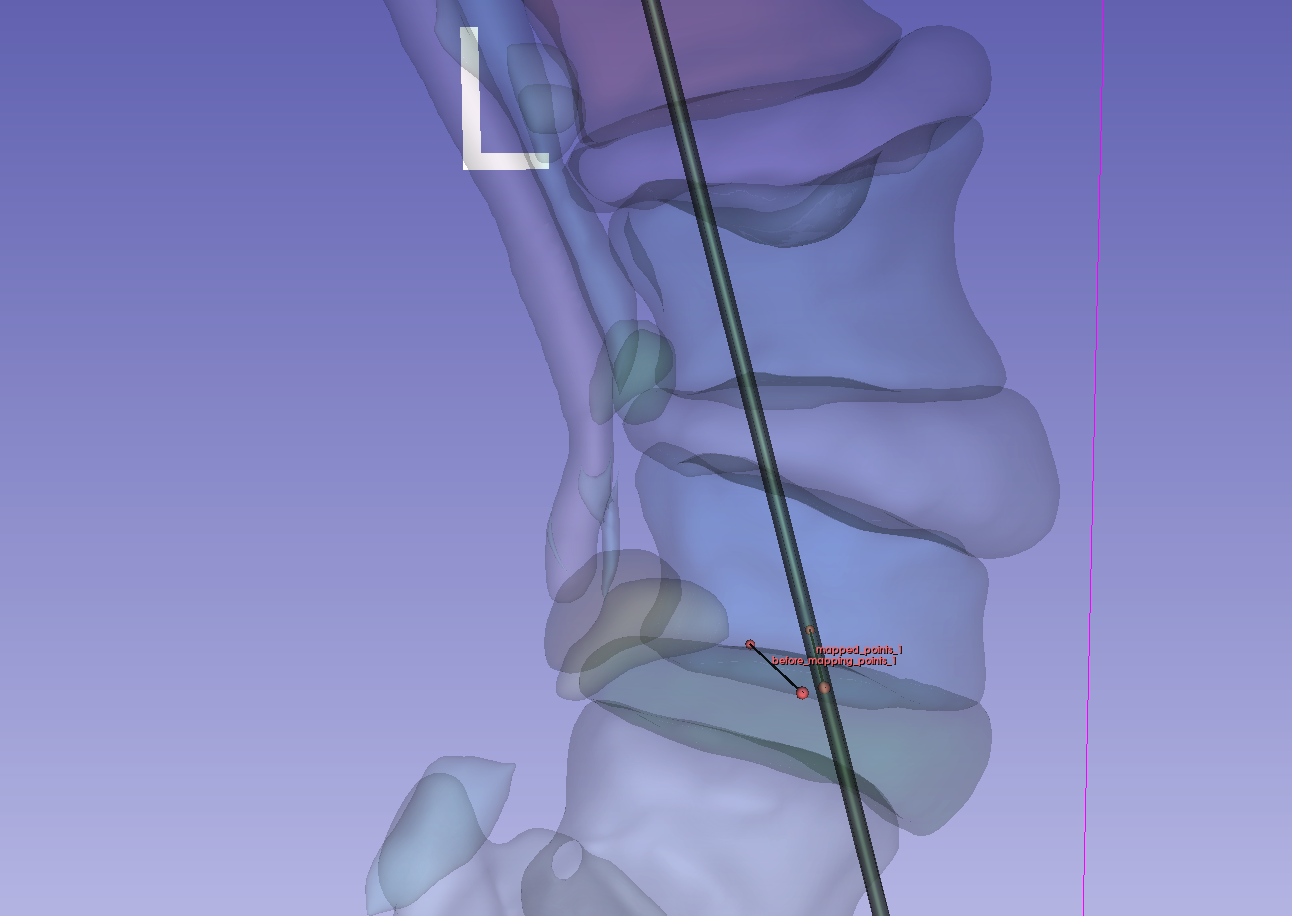
\includegraphics[width=\textwidth]{obrazy/after_mapping_to_common_plane_lower.png}
    \caption{Widok boczny}
    \label{fig:lower_common_plane}
    \end{subfigure}
    \hfill
    \begin{subfigure}[b]{0.48\textwidth}
    \centering
    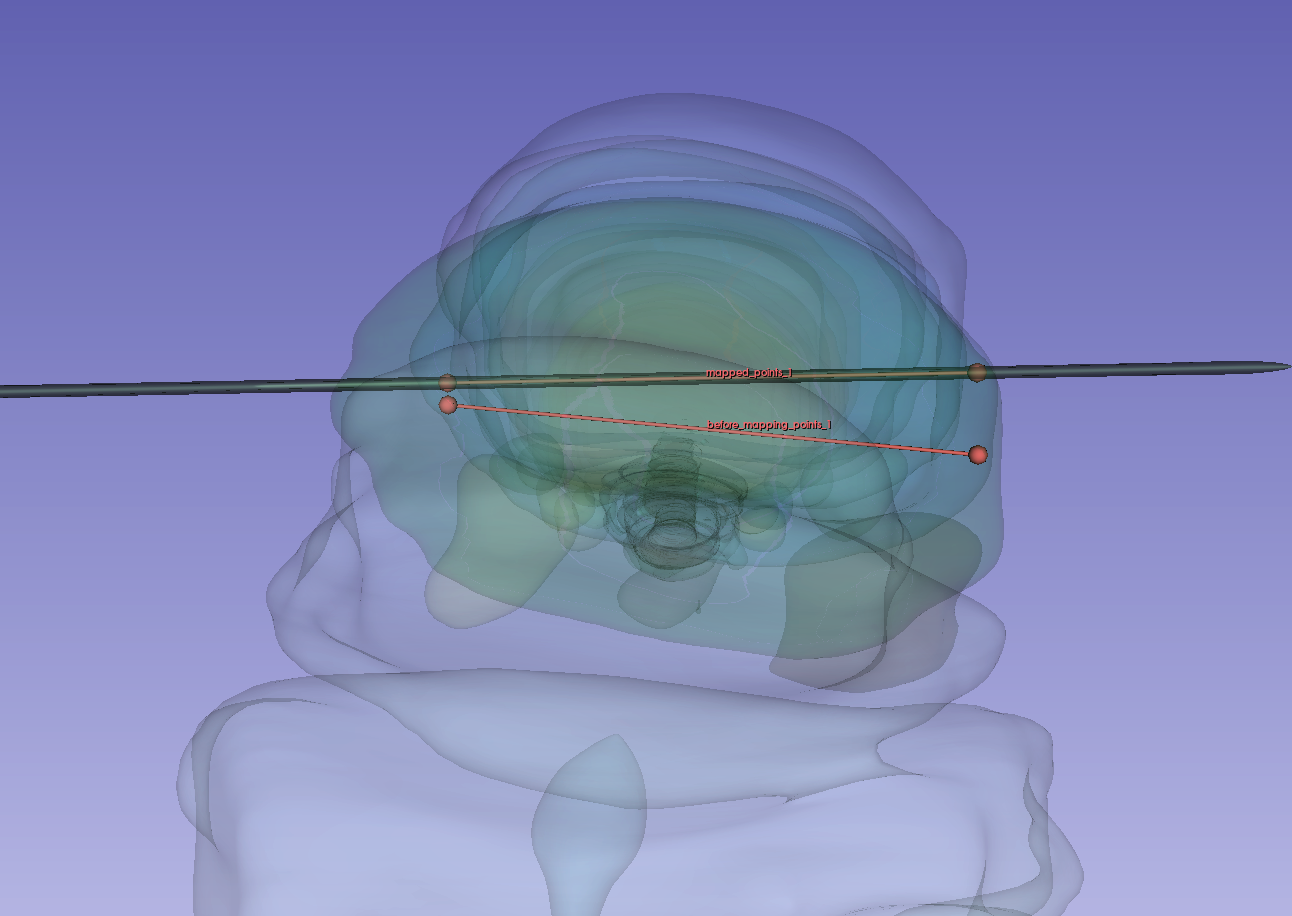
\includegraphics[width=\textwidth]{obrazy/after_mapping_to_common_plane_upper.png}
    \caption{Widok dolny}
    \label{fig:upper_common_plane}
    \end{subfigure}
    \caption{Przestrzenna wizualizacja wyników rzutowania punktów kręgu na wspólną płaszczyznę analizowanej pary kręgów.}
\end{figure}


Po rzutowaniu punktów na optymalną płaszczyznę, algorytm implementuje funkcję \texttt{cobb\_angle}, której zadaniem jest wyznaczenie kąta pomiędzy wektorami reprezentującymi krawędzie kręgów granicznych oraz określenie orientacji skrzywienia (lewo- lub prawostronne).
Dla wybranej pary kręgów definiowane są dwa wektory kierunkowe $u$ (wektor krawędzi górnej kręgu górnego) oraz $l$ (wektor krawędzi dolnej kręgu dolnego).
Zgodnie z geometryczną implementacją metody Cobba, kąt skrzywienia $\alpha$ odpowiada kątowi przecięcia prostych zawierających te wektory.
Wartość kąta wyznaczana jest przy użyciu iloczynu skalarnego:
\begin{equation} \label{eq:cobb}
\begin{aligned}
    \vec{v}_1 \cdot \vec{v}_2 &= x_1 x_2 + y_1 y_2 \\
    \|\vec{v}_1\| &= \sqrt{x_1^2 + y_1^2}, \quad \|\vec{v}_2\| = \sqrt{x_2^2 + y_2^2} \\
    \alpha &= \arccos\!\left(\frac{\vec{v}_1 \cdot \vec{v}_2}{\|\vec{v}_1\|\,\|\vec{v}_2\|}\right) \cdot \frac{180\degree}{\pi}
\end{aligned}
\end{equation}

Aby zapewnić poprawność obliczeń niezależnie od orientacji kręgosłupa w globalnym układzie współrzędnych skanera, wektory $\vec{v}_1$ i $\vec{v}_2$ są przed obliczeniem kąta rzutowane na dwuwymiarowy układ współrzędnych wspólnej płaszczyzny pomiarowej, wyznaczonej przez bazy $\vec{x}_{plane}$ i $\vec{y}_{plane}$ (wyznaczone wcześniej metodą SVD):

\begin{equation}
    \vec{u}_k = \begin{bmatrix} \vec{v}_k \cdot \vec{x}_{plane} \\ \vec{v}_k \cdot \vec{y}_{plane} \end{bmatrix}, \quad k \in \{1, 2\}
\end{equation}

Operacja ta eliminuje składową normalną do płaszczyzny, zapewniając, że iloczyn skalarny i normy w równaniu \eqref{eq:cobb} operują wyłącznie na geometrii leżącej w płaszczyźnie pomiaru.

Strona skrzywienia kręgosłupa wyznaczana jest na podstawie znaku iloczynu wektorowego rzutowanych wektorów $\vec{u}_1$ i $\vec{u}_2$:

\begin{equation} \label{eq:cross_sign}
    c = u_{1x} \cdot u_{2y} - u_{1y} \cdot u_{2x}
\end{equation}

Jeżeli $c \geq 0$, skrzywienie klasyfikowane jest jako \textit{prawostronne} (łac. \textit{dextroscoliosis}), w przeciwnym razie jako \textit{lewostronne} (łac. \textit{levoscoliosis}).

Obliczenia kąta Cobba wykonywane są dla wszystkich par kręgów $(k_i,\, k_j)$ spełniających warunek $j \geq i + 2$, co wyklucza pary kręgów bezpośrednio sąsiadujących i odpowiada klinicznej definicji skrzywienia angażującego co najmniej trzy poziomy kręgosłupa. Wynikowy kąt maksymalny wyznaczany jest jako:

\begin{equation} \label{eq:max_cobb}
    \alpha_{max} = \max_{\substack{i,j \\ j \geq i+2}} |\alpha(k_i, k_j)|
\end{equation}

Wynikiem działania algorytmu jest wartość kąta Cobba wyrażona w stopniach, para kręgów wyznaczająca największą deformację oraz strona skrzywienia (prawostronna lub lewostronna). Dane pośrednie - punkty kanału kręgowego, wektory lokalnych układów współrzędnych oraz punkty narożne trzonów - są eksportowane do plików JSON kompatybilnych z oprogramowaniem 3D Slicer, co umożliwia wizualną weryfikację wyników przez lekarza.